% \begin{appendices}
% 	\crefalias{chapter}{appcha}
% 	\crefalias{section}{appsec}
% 	\renewcommand{\thesection}{\Alph{chapter}\arabic{section}}

	\chapter{Additional results from \cref{cha:obesity_associated_genetic_signature_and_pathway_signatures}}
	\label{app:b}

	\section{Ranking method for the pathway-associated genetic signatures}
	\label{sec:ranking_method_for_the_pathway_associated_genetic_signatures}

	To determine whether it was the best to rank the metagene scores based on the number of samples or rank the scores with the probit method, the two ranking methods were compared in scatter plots with the GT pathway metagenes in \gls{rma} or \gls{mas} normalised GT data.
	Since the results from the \gls{rma} and \gls{mas} normalised GT data were so similar to one another, only the results from the \gls{rma} normalised data are presented (\cref{fig:appendix/rank_scatter}).
	\cref{fig:appendix/rank_scatter} showed that the metagene scores for all of the GT pathway-associated genetic signatures were approximately the same in either of the ranking methods used.

	\begin{figure}[htp!]
		\centering
		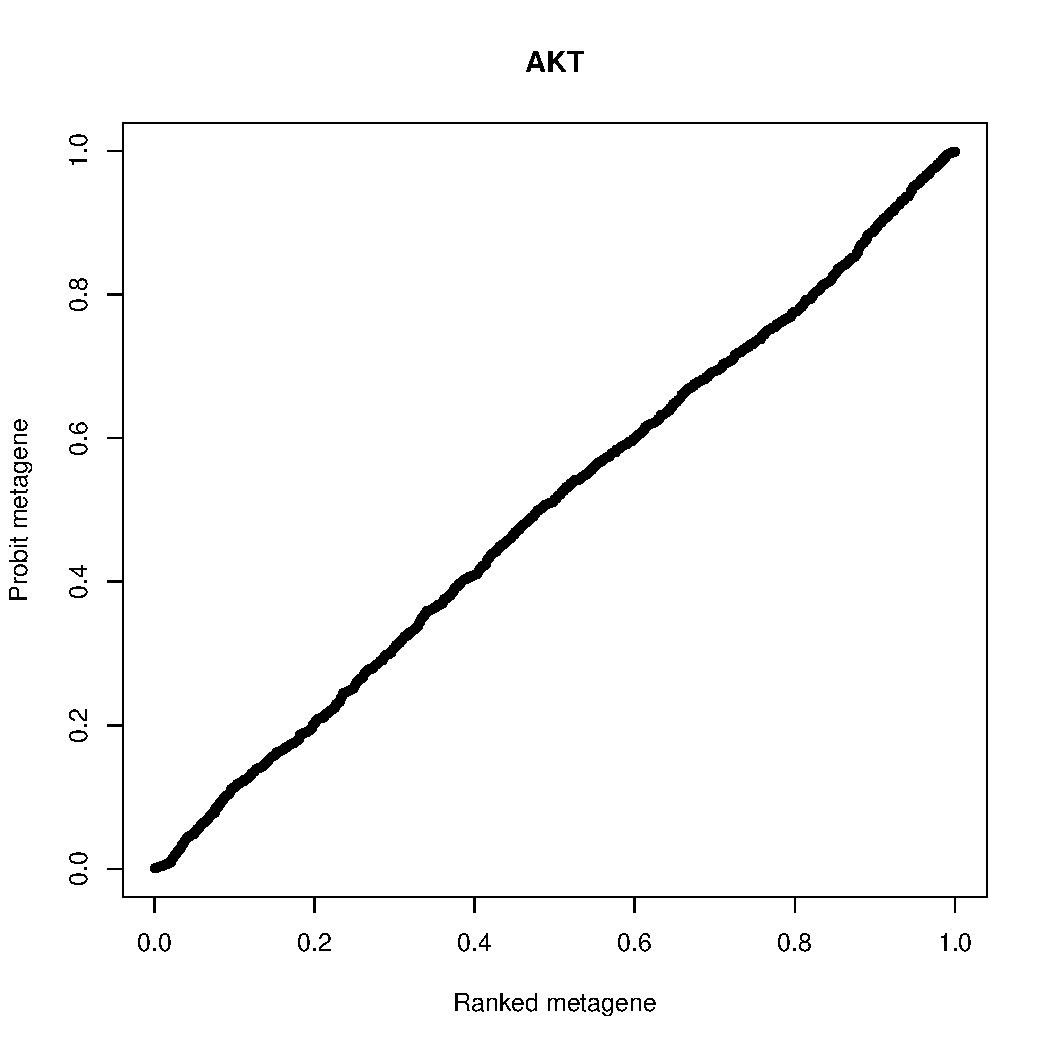
\includegraphics[width=0.32\linewidth,page=1]{appendix/gatza_rma_meta_rank_vs_probit}
		\includegraphics[width=0.32\linewidth,page=2]{appendix/gatza_rma_meta_rank_vs_probit}
		\includegraphics[width=0.32\linewidth,page=3]{appendix/gatza_rma_meta_rank_vs_probit}\\
		\includegraphics[width=0.32\linewidth,page=4]{appendix/gatza_rma_meta_rank_vs_probit}
		\includegraphics[width=0.32\linewidth,page=5]{appendix/gatza_rma_meta_rank_vs_probit}
		\includegraphics[width=0.32\linewidth,page=6]{appendix/gatza_rma_meta_rank_vs_probit}\\
		\includegraphics[width=0.32\linewidth,page=7]{appendix/gatza_rma_meta_rank_vs_probit}
		\includegraphics[width=0.32\linewidth,page=8]{appendix/gatza_rma_meta_rank_vs_probit}
		\includegraphics[width=0.32\linewidth,page=9]{appendix/gatza_rma_meta_rank_vs_probit}\\
		\includegraphics[width=0.32\linewidth,page=10]{appendix/gatza_rma_meta_rank_vs_probit}
		\includegraphics[width=0.32\linewidth,page=11]{appendix/gatza_rma_meta_rank_vs_probit}
		\includegraphics[width=0.32\linewidth,page=12]{appendix/gatza_rma_meta_rank_vs_probit}\\
		\caption[Comparison of the ranking methods for the pathway metagenes in the \acrshort{rma}-normalised GT data]{Scatter plots comparing the GT pathway metagenes ranked with probit and ranked based on number of samples in \gls{rma} normalised GT data. }
		\label{fig:appendix/rank_scatter}
	\end{figure}

	\begin{figure}[htpb]
		\ContinuedFloat
		\captionsetup{list=off,format=cont}
		\centering
		\includegraphics[width=0.32\linewidth,page=13]{appendix/gatza_rma_meta_rank_vs_probit}
		\includegraphics[width=0.32\linewidth,page=14]{appendix/gatza_rma_meta_rank_vs_probit}
		\includegraphics[width=0.32\linewidth,page=15]{appendix/gatza_rma_meta_rank_vs_probit}\\
		\includegraphics[width=0.32\linewidth,page=16]{appendix/gatza_rma_meta_rank_vs_probit}
		\includegraphics[width=0.32\linewidth,page=17]{appendix/gatza_rma_meta_rank_vs_probit}
		\includegraphics[width=0.32\linewidth,page=18]{appendix/gatza_rma_meta_rank_vs_probit}\\
		\vspace{1em}
		\caption[]{figure}
	\end{figure}

	\section{Normalisation method for the pathway-associated genetic signature transformation matrices}
	\label{sec:normalisation_method_for_pathway_associated_genetic_signature_transformation_matrices}

	To investigate whether the normalisation methods were important in the creation of the pathway-associated genetic signature transformation matrices, and whether the normalisation methods of the data affected the resulting metagenes, transformation matrices were generated in \gls{rma} or \gls{mas} normalised GT data set and then applied to the \gls{rma} or \gls{mas} normalised GT data set.
	The results in \cref{fig:appendix/gt_meta_rma_mas} showed less variability of the metagene scores when the metagenes were derived from the data with the same normalisation method, regardless of the transformation matrix used to produce the metagenes.
	This was most clearly demonstrated by the \gls{bcat}, \gls{er}, \gls{ifna}, \gls{ifny}, p53 and \gls{pr} pathway-associated genetic signatures.

	As mentioned in \cref{sec:pathway_associated_genetic_signatures_from_gatza2010a_study} some of the pathway metagenes showed greater variability than the other pathway metagene scores.
	This was also seen in other data sets as well (only the \gls{pr} and \gls{tgfb} metagenes shown; \cref{fig:appendix/gt_meta_rma_mas_other_data}).

	\begin{figure}[htp!]
		\centering
		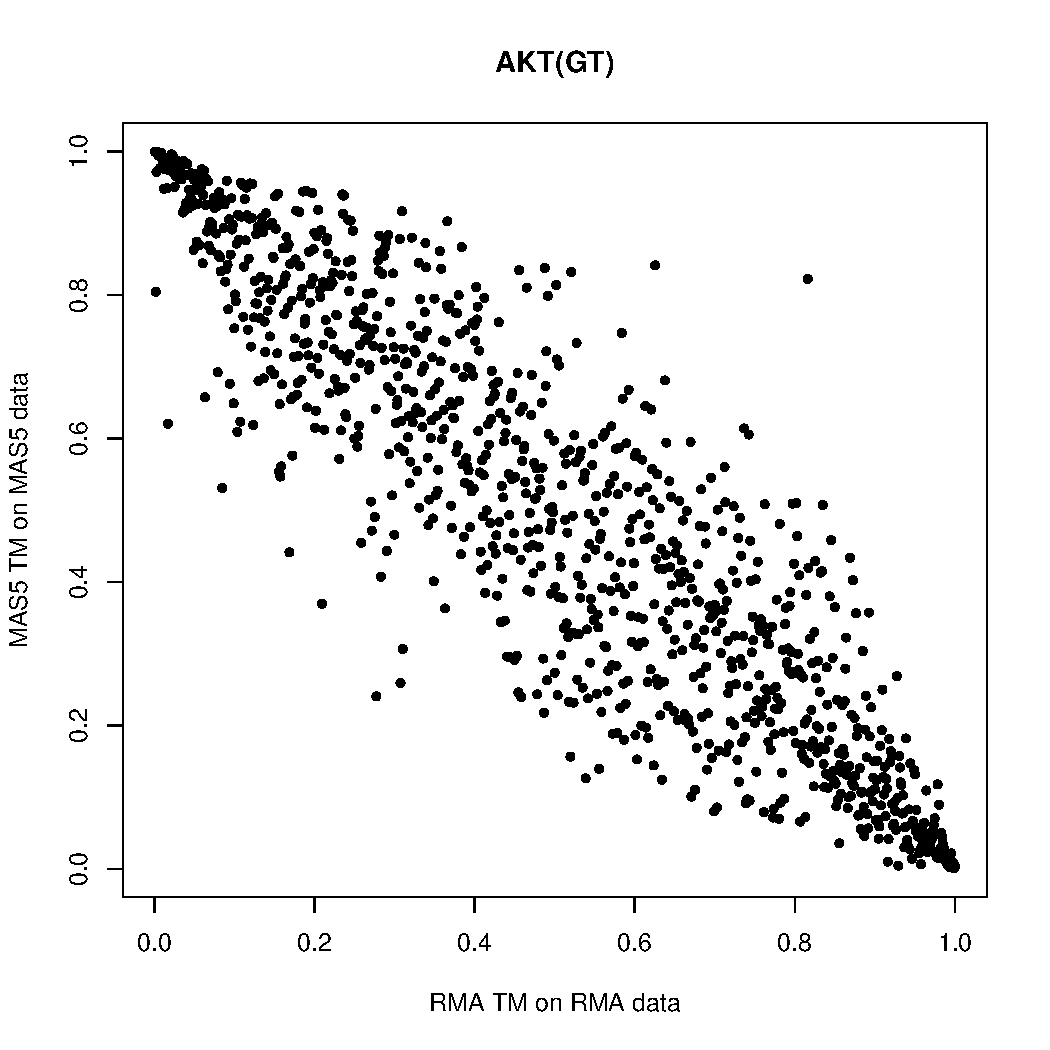
\includegraphics[width=0.32\linewidth,page=1]{appendix/allmeta_rma_vs_mas}
		\includegraphics[width=0.32\linewidth,page=2]{appendix/allmeta_rma_vs_mas}
		\includegraphics[width=0.32\linewidth,page=3]{appendix/allmeta_rma_vs_mas}\\
		\includegraphics[width=0.32\linewidth,page=4]{appendix/allmeta_rma_vs_mas}
		\includegraphics[width=0.32\linewidth,page=5]{appendix/allmeta_rma_vs_mas}
		\includegraphics[width=0.32\linewidth,page=6]{appendix/allmeta_rma_vs_mas}\\
		\includegraphics[width=0.32\linewidth,page=7]{appendix/allmeta_rma_vs_mas}
		\includegraphics[width=0.32\linewidth,page=8]{appendix/allmeta_rma_vs_mas}
		\includegraphics[width=0.32\linewidth,page=9]{appendix/allmeta_rma_vs_mas}\\
		\includegraphics[width=0.32\linewidth,page=10]{appendix/allmeta_rma_vs_mas}
		\includegraphics[width=0.32\linewidth,page=11]{appendix/allmeta_rma_vs_mas}
		\includegraphics[width=0.32\linewidth,page=12]{appendix/allmeta_rma_vs_mas}\\
		\caption[Comparison of the normalisation methods used for the pathway metagene TM and the GT data]{Scatter plots comparing the GT pathway metagenes derived from the transformation matrices in \gls{rma}- or \gls{mas}-normalised GT data set.
		All of the transformation matrices were generated in either the \gls{rma} or \gls{mas} normalised GT data set.
		}
		\label{fig:appendix/gt_meta_rma_mas}
	\end{figure}

	\begin{figure}[htpb]
		\ContinuedFloat
		\captionsetup{list=off,format=cont}
		\centering
		\includegraphics[width=0.32\linewidth,page=13]{appendix/allmeta_rma_vs_mas}
		\includegraphics[width=0.32\linewidth,page=14]{appendix/allmeta_rma_vs_mas}
		\includegraphics[width=0.32\linewidth,page=15]{appendix/allmeta_rma_vs_mas}\\
		\includegraphics[width=0.32\linewidth,page=16]{appendix/allmeta_rma_vs_mas}
		\includegraphics[width=0.32\linewidth,page=17]{appendix/allmeta_rma_vs_mas}
		\includegraphics[width=0.32\linewidth,page=18]{appendix/allmeta_rma_vs_mas}\\
		\includegraphics[width=0.32\linewidth,page=19]{appendix/allmeta_rma_vs_mas}
		\includegraphics[width=0.32\linewidth,page=20]{appendix/allmeta_rma_vs_mas}
		\includegraphics[width=0.32\linewidth,page=21]{appendix/allmeta_rma_vs_mas}\\
		\includegraphics[width=0.32\linewidth,page=22]{appendix/allmeta_rma_vs_mas}
		\includegraphics[width=0.32\linewidth,page=23]{appendix/allmeta_rma_vs_mas}
		\includegraphics[width=0.32\linewidth,page=24]{appendix/allmeta_rma_vs_mas}\\
		\caption[]{figure}
	\end{figure}

	\begin{figure}[htpb]
		\ContinuedFloat
		\captionsetup{list=off,format=cont}
		\centering
		\includegraphics[width=0.32\linewidth,page=25]{appendix/allmeta_rma_vs_mas}
		\includegraphics[width=0.32\linewidth,page=26]{appendix/allmeta_rma_vs_mas}
		\includegraphics[width=0.32\linewidth,page=27]{appendix/allmeta_rma_vs_mas}\\
		\includegraphics[width=0.32\linewidth,page=28]{appendix/allmeta_rma_vs_mas}
		\includegraphics[width=0.32\linewidth,page=29]{appendix/allmeta_rma_vs_mas}
		\includegraphics[width=0.32\linewidth,page=30]{appendix/allmeta_rma_vs_mas}\\
		\includegraphics[width=0.32\linewidth,page=31]{appendix/allmeta_rma_vs_mas}
		\includegraphics[width=0.32\linewidth,page=32]{appendix/allmeta_rma_vs_mas}
		\includegraphics[width=0.32\linewidth,page=33]{appendix/allmeta_rma_vs_mas}\\
		\includegraphics[width=0.32\linewidth,page=34]{appendix/allmeta_rma_vs_mas}
		\includegraphics[width=0.32\linewidth,page=35]{appendix/allmeta_rma_vs_mas}
		\includegraphics[width=0.32\linewidth,page=36]{appendix/allmeta_rma_vs_mas}\\
		\caption[]{figure}
	\end{figure}
	
	\begin{figure}[htpb]
		\ContinuedFloat
		\captionsetup{list=off,format=cont}
		\centering
		\includegraphics[width=0.32\linewidth,page=37]{appendix/allmeta_rma_vs_mas}
		\includegraphics[width=0.32\linewidth,page=38]{appendix/allmeta_rma_vs_mas}
		\includegraphics[width=0.32\linewidth,page=39]{appendix/allmeta_rma_vs_mas}\\
		\includegraphics[width=0.32\linewidth,page=40]{appendix/allmeta_rma_vs_mas}
		\includegraphics[width=0.32\linewidth,page=41]{appendix/allmeta_rma_vs_mas}
		\includegraphics[width=0.32\linewidth,page=42]{appendix/allmeta_rma_vs_mas}\\
		\includegraphics[width=0.32\linewidth,page=43]{appendix/allmeta_rma_vs_mas}
		\includegraphics[width=0.32\linewidth,page=44]{appendix/allmeta_rma_vs_mas}
		\includegraphics[width=0.32\linewidth,page=45]{appendix/allmeta_rma_vs_mas}\\
		\includegraphics[width=0.32\linewidth,page=46]{appendix/allmeta_rma_vs_mas}
		\includegraphics[width=0.32\linewidth,page=47]{appendix/allmeta_rma_vs_mas}
		\includegraphics[width=0.32\linewidth,page=48]{appendix/allmeta_rma_vs_mas}\\
		\caption[]{figure}
	\end{figure}
	
	\begin{figure}[htpb]
		\ContinuedFloat
		\captionsetup{list=off,format=cont}
		\centering
		\includegraphics[width=0.32\linewidth,page=49]{appendix/allmeta_rma_vs_mas}
		\includegraphics[width=0.32\linewidth,page=50]{appendix/allmeta_rma_vs_mas}
		\includegraphics[width=0.32\linewidth,page=51]{appendix/allmeta_rma_vs_mas}\\
		\includegraphics[width=0.32\linewidth,page=52]{appendix/allmeta_rma_vs_mas}
		\includegraphics[width=0.32\linewidth,page=53]{appendix/allmeta_rma_vs_mas}
		\includegraphics[width=0.32\linewidth,page=54]{appendix/allmeta_rma_vs_mas}\\
		\includegraphics[width=0.32\linewidth,page=55]{appendix/allmeta_rma_vs_mas}
		\includegraphics[width=0.32\linewidth,page=56]{appendix/allmeta_rma_vs_mas}
		\includegraphics[width=0.32\linewidth,page=57]{appendix/allmeta_rma_vs_mas}\\
		\includegraphics[width=0.32\linewidth,page=58]{appendix/allmeta_rma_vs_mas}
		\includegraphics[width=0.32\linewidth,page=59]{appendix/allmeta_rma_vs_mas}
		\includegraphics[width=0.32\linewidth,page=60]{appendix/allmeta_rma_vs_mas}\\
		\caption[]{figure}
	\end{figure}
	
	\begin{figure}[htpb]
		\ContinuedFloat
		\captionsetup{list=off,format=cont}
		\centering
		\includegraphics[width=0.32\linewidth,page=61]{appendix/allmeta_rma_vs_mas}
		\includegraphics[width=0.32\linewidth,page=62]{appendix/allmeta_rma_vs_mas}
		\includegraphics[width=0.32\linewidth,page=63]{appendix/allmeta_rma_vs_mas}\\
		\includegraphics[width=0.32\linewidth,page=64]{appendix/allmeta_rma_vs_mas}
		\includegraphics[width=0.32\linewidth,page=65]{appendix/allmeta_rma_vs_mas}
		\includegraphics[width=0.32\linewidth,page=66]{appendix/allmeta_rma_vs_mas}\\
		\includegraphics[width=0.32\linewidth,page=67]{appendix/allmeta_rma_vs_mas}
		\includegraphics[width=0.32\linewidth,page=68]{appendix/allmeta_rma_vs_mas}
		\includegraphics[width=0.32\linewidth,page=69]{appendix/allmeta_rma_vs_mas}\\
		\includegraphics[width=0.32\linewidth,page=70]{appendix/allmeta_rma_vs_mas}
		\includegraphics[width=0.32\linewidth,page=71]{appendix/allmeta_rma_vs_mas}
		\includegraphics[width=0.32\linewidth,page=72]{appendix/allmeta_rma_vs_mas}\\
		\caption[]{figure}
	\end{figure}
	
	\begin{figure}[htpb]
		\ContinuedFloat
		\captionsetup{list=off,format=cont}
		\centering
		\includegraphics[width=0.32\linewidth,page=73]{appendix/allmeta_rma_vs_mas}
		\includegraphics[width=0.32\linewidth,page=74]{appendix/allmeta_rma_vs_mas}
		\includegraphics[width=0.32\linewidth,page=75]{appendix/allmeta_rma_vs_mas}\\
		\includegraphics[width=0.32\linewidth,page=76]{appendix/allmeta_rma_vs_mas}
		\includegraphics[width=0.32\linewidth,page=77]{appendix/allmeta_rma_vs_mas}
		\includegraphics[width=0.32\linewidth,page=78]{appendix/allmeta_rma_vs_mas}\\
		\includegraphics[width=0.32\linewidth,page=79]{appendix/allmeta_rma_vs_mas}
		\includegraphics[width=0.32\linewidth,page=80]{appendix/allmeta_rma_vs_mas}
		\includegraphics[width=0.32\linewidth,page=81]{appendix/allmeta_rma_vs_mas}\\
		\includegraphics[width=0.32\linewidth,page=82]{appendix/allmeta_rma_vs_mas}
		\includegraphics[width=0.32\linewidth,page=83]{appendix/allmeta_rma_vs_mas}
		\includegraphics[width=0.32\linewidth,page=84]{appendix/allmeta_rma_vs_mas}\\
		\caption[]{figure}
	\end{figure}

	\begin{figure}[htpb]
		\ContinuedFloat
		\captionsetup{list=off,format=cont}
		\centering
		\includegraphics[width=0.32\linewidth,page=85]{appendix/allmeta_rma_vs_mas}
		\includegraphics[width=0.32\linewidth,page=86]{appendix/allmeta_rma_vs_mas}
		\includegraphics[width=0.32\linewidth,page=87]{appendix/allmeta_rma_vs_mas}\\
		\includegraphics[width=0.32\linewidth,page=88]{appendix/allmeta_rma_vs_mas}
		\includegraphics[width=0.32\linewidth,page=89]{appendix/allmeta_rma_vs_mas}
		\includegraphics[width=0.32\linewidth,page=90]{appendix/allmeta_rma_vs_mas}\\
		\includegraphics[width=0.32\linewidth,page=91]{appendix/allmeta_rma_vs_mas}
		\includegraphics[width=0.32\linewidth,page=92]{appendix/allmeta_rma_vs_mas}
		\includegraphics[width=0.32\linewidth,page=93]{appendix/allmeta_rma_vs_mas}\\
		\includegraphics[width=0.32\linewidth,page=94]{appendix/allmeta_rma_vs_mas}
		\includegraphics[width=0.32\linewidth,page=95]{appendix/allmeta_rma_vs_mas}
		\includegraphics[width=0.32\linewidth,page=96]{appendix/allmeta_rma_vs_mas}\\
		\caption[]{figure}
	\end{figure}
	
	\begin{figure}[htpb]
		\ContinuedFloat
		\captionsetup{list=off,format=cont}
		\centering
		\includegraphics[width=0.32\linewidth,page=97]{appendix/allmeta_rma_vs_mas}
		\includegraphics[width=0.32\linewidth,page=98]{appendix/allmeta_rma_vs_mas}
		\includegraphics[width=0.32\linewidth,page=99]{appendix/allmeta_rma_vs_mas}\\
		\includegraphics[width=0.32\linewidth,page=100]{appendix/allmeta_rma_vs_mas}
		\includegraphics[width=0.32\linewidth,page=101]{appendix/allmeta_rma_vs_mas}
		\includegraphics[width=0.32\linewidth,page=102]{appendix/allmeta_rma_vs_mas}\\
		\includegraphics[width=0.32\linewidth,page=103]{appendix/allmeta_rma_vs_mas}
		\includegraphics[width=0.32\linewidth,page=104]{appendix/allmeta_rma_vs_mas}
		\includegraphics[width=0.32\linewidth,page=105]{appendix/allmeta_rma_vs_mas}\\
		\includegraphics[width=0.32\linewidth,page=106]{appendix/allmeta_rma_vs_mas}
		\includegraphics[width=0.32\linewidth,page=107]{appendix/allmeta_rma_vs_mas}
		\includegraphics[width=0.32\linewidth,page=108]{appendix/allmeta_rma_vs_mas}\\
		\caption[]{figure}
	\end{figure}

	\begin{figure}[htp!]
		\centering
		\includegraphics[width=0.32\linewidth,page=244]{appendix/allmeta_rma_vs_mas}
		\includegraphics[width=0.32\linewidth,page=412]{appendix/allmeta_rma_vs_mas}
		\includegraphics[width=0.32\linewidth,page=580]{appendix/allmeta_rma_vs_mas}\\
		\includegraphics[width=0.32\linewidth,page=268]{appendix/allmeta_rma_vs_mas}
		\includegraphics[width=0.32\linewidth,page=436]{appendix/allmeta_rma_vs_mas}
		\includegraphics[width=0.32\linewidth,page=604]{appendix/allmeta_rma_vs_mas}
		\caption[Comparison of the pathway metagenes generated in the \acrshort{mas} normalised CR, FM and \gls{nzbc} data sets from the application of the transformation matrices derived from either the \acrshort{rma} or \acrshort{mas} normalised GT data]{Comparison of the pathway metagenes generated in the \acrshort{mas} normalised CR, FM and \gls{nzbc} data sets from the application of the transformation matrices derived from either the \acrshort{rma} or \acrshort{mas} normalised GT data.
	Only the \gls{pr} (top) and the \gls{tgfb}  (bottom) pathway metagenes are shown, due to the large number of scatter plots generated.
	}
		\label{fig:appendix/gt_meta_rma_mas_other_data}
	\end{figure}

	\newpage


	\section{Additional results used to determine the directionality of the pathway metagenes}
	\label{sec:additional_results_to_determine_the_directionality_of_the_pathway_metagenes}

	The directionality of the pathway metagenes were determined by comparing the metagene values with the gene expression of the representative gene for the pathway-associated genetic signature, as well as the gene expression pattern of the pathway signature (\cref{fig:appendix/gt_pathmeta_rank}).
	Together with the original results presented by \citet{Gatza2010a} (\cref{sec:result_from_gatza2010a_study}), the final directions of the pathway metagenes were decided.

	\begin{figure}[htp!]
		\centering
		\includegraphics[width=0.32\linewidth,page=1]{appendix/gtrmastdrank}
		\includegraphics[width=0.32\linewidth,page=2]{appendix/gtrmastdrank}
		\includegraphics[width=0.32\linewidth,page=3]{appendix/gtrmastdrank}\\
		\includegraphics[width=0.32\linewidth,page=4]{appendix/gtrmastdrank}
		\includegraphics[width=0.32\linewidth,page=5]{appendix/gtrmastdrank}
		\includegraphics[width=0.32\linewidth,page=6]{appendix/gtrmastdrank}\\
		\caption[Directionality of the pathway metagenes in the GT data]{Heatmaps showing the gene expression of the pathway-associated genetic signatures, pathway metagenes, and the expression of the representative pathway gene in \gls{rma}-normalised GT data set.
		For each pathway-associated genetic signature, the gene expression pattern of the signature was plotted in the heatmap.
		The expression of the representative gene for the pathway signature (see \cref{tab:metagene_direction} in \cref{sub:metagene_direction}) was plotted seaparately as a bar above the pathway metagene scores.
		}
		\label{fig:appendix/gt_pathmeta_rank}
	\end{figure}

	\begin{figure}[htpb]
		\ContinuedFloat
		\captionsetup{list=off,format=cont}
		\centering
		\includegraphics[width=0.32\linewidth,page=7]{appendix/gtrmastdrank}
		\includegraphics[width=0.32\linewidth,page=8]{appendix/gtrmastdrank}
		\includegraphics[width=0.32\linewidth,page=9]{appendix/gtrmastdrank}\\
		\includegraphics[width=0.32\linewidth,page=10]{appendix/gtrmastdrank}
		\includegraphics[width=0.32\linewidth,page=11]{appendix/gtrmastdrank}
		\includegraphics[width=0.32\linewidth,page=12]{appendix/gtrmastdrank}\\
		\includegraphics[width=0.32\linewidth,page=13]{appendix/gtrmastdrank}
		\includegraphics[width=0.32\linewidth,page=14]{appendix/gtrmastdrank}
		\includegraphics[width=0.32\linewidth,page=15]{appendix/gtrmastdrank}\\
		\includegraphics[width=0.32\linewidth,page=16]{appendix/gtrmastdrank}
		\includegraphics[width=0.32\linewidth,page=17]{appendix/gtrmastdrank}
		\includegraphics[width=0.32\linewidth,page=18]{appendix/gtrmastdrank}\\
		\caption[]{figure}
	\end{figure}

	\newpage

	\section{Original result from the \citet{Gatza2010a} study}
	\label{sec:result_from_gatza2010a_study}

	The original result from the \citet{Gatza2010a} study were used to determine the directions of the GT pathway-associated genetic signatures in \cref{sec:pathway_associated_genetic_signatures_from_gatza2010a_study} (\cref{fig:gatza_paper_res}).

	\begin{figure}[htpb]
		\centering
		\includegraphics[width=0.7\linewidth]{results2/gatzares1}
		\caption[Original result presented in the \citet{Gatza2010a} study]{Heatmap showing the correlation of all of the GT pathway-associated genetic signatures with one another.
		Figure adapted from the \citet{Gatza2010a} study.}
		\label{fig:gatza_paper_res}
	\end{figure}

	\section{Correlation of the GT pathway metagenes in other cancer data sets}
	\label{sec:correlation_of_the_gt_pathway_metagenes_in_other_cancer_data_sets}

	The correlation of the pathway-associated genetic signatures were plotted as heatmaps for the CR, FM and \gls{nzbc} data sets to confirm that the pathway transformation matrices from the GT data set were generating metagenes that were similar to those in the original \gls{rma} normalised GT data.
	Most importantly, the pathway metagenes generated from the transformation matrices had to cluster in a similar pattern as the pathway metagenes in the GT data set.
	This was to confirm that the directionality of the metagenes were conserved even after the transformation matrices were applied to the data set

	\begin{figure}[htp!]
		\centering
		\includegraphics[width=0.65\linewidth,page=3]{appendix/gatza_meta_trans}
		\includegraphics[width=0.65\linewidth,page=7]{appendix/gatza_meta_trans}
		\caption[Heatmaps of the Pearson correlation of all the pathway metagenes in the \gls{rma}-normalised CR, \gls{nzbc} and FM data]{Heatmaps showing the correlation of all of the pathway metagenes with one another in \gls{rma} normalised CR, \gls{nzbc} and FM data sets.
		High and low correlation were represented as red and blue, respectively, where the colours were matched with the values on the scale shown in the top left histogram.}
		\label{fig:appendix/gt_pathmeta_other_data}
	\end{figure}

	\begin{figure}[htpb]
		\ContinuedFloat
		\captionsetup{list=off,format=cont}
		\centering
		\includegraphics[width=0.7\linewidth,page=11]{appendix/gatza_meta_trans}
		\caption[]{figure}
	\end{figure}

	\section{Directionality of the obesity metagenes in the GT data}
	\label{sec:directionality_of_the_obesity_metagenes_in_the_gt_data}

	The directionality of the CR obesity-associated genetic signatures were determined in the \gls{rma} normalised GT data set to make sure these signatures were in the ``correct'' direction, and therefore able to be compared with the pathway-associated genetic signatures appropriately.
	As clearly shown in \cref{fig:appendix/ob_meta_dir_gt}, the Res metagene was flipped as the Res metagene was in the oppsite direction compared with the other obesity metagenes.

	\begin{figure}[htp!]
		\centering
		\includegraphics[width=0.32\linewidth,page=1]{appendix/gtobrma}
		\includegraphics[width=0.32\linewidth,page=2]{appendix/gtobrma}
		\includegraphics[width=0.32\linewidth,page=3]{appendix/gtobrma}\\
		\includegraphics[width=0.32\linewidth,page=4]{appendix/gtobrma}
		\includegraphics[width=0.32\linewidth,page=5]{appendix/gtobrma}
		\includegraphics[width=0.32\linewidth,page=6]{appendix/gtobrma}\\
		\includegraphics[width=0.32\linewidth,page=7]{appendix/gtobrma}
		\includegraphics[width=0.32\linewidth,page=8]{appendix/gtobrma}
		\includegraphics[width=0.32\linewidth,page=9]{appendix/gtobrma}\\
		\caption[Heatmaps of all the obesity and the pathway metagenes in the CR, \gls{nzbc} and FM data]{Heatmaps showing the obesity metagenes from the CR data set with the gene expressions of the obesity-associated genetic signatures in the \gls{rma} normalised GT data set.
		High and low correlation were represented as red and blue, respectively, where the colours were matched with the values on the scale shown in the top left histogram.}
		\label{fig:appendix/ob_meta_dir_gt}
	\end{figure}

	\newpage

	\section{Visual comparison of the correlation of \gls{svd} and TM generated pathway metagenes}
	\label{sec:comparison_of_the_correlation_of_svd_and_tm_generated_pathway_metagenes}

	This section provides visual comparison of the Spearman correlation of the \gls{svd}- and TM-generated pathway and obesity metagenes in the CR, FM, GT and \gls{nzbc} data sets (\cref{fig:allmetacor_bar_appendix}).
	The Akt, \gls{egfr}, \gls{her2}, p53, p63, \gls{pi3k}, Ras, Src, \gls{stat3}, \gls{tgfb} and \gls{tnfa} pathway signatures showed a correlation of 0.8 or less in at least one of the four data sets.

	\begin{figure}[htpb]
		\centering
		\includegraphics[width=0.24\linewidth,page=1]{results2/allmetacor_bar}
		\includegraphics[width=0.24\linewidth,page=2]{results2/allmetacor_bar}
		\includegraphics[width=0.24\linewidth,page=3]{results2/allmetacor_bar}
		\includegraphics[width=0.24\linewidth,page=4]{results2/allmetacor_bar}\\
		\caption[Bar plots showing the Spearman correlation of the \gls{svd}- and TM-derived obesity and pathway metagenes across different data sets]{Visual comparison of the Spearman correlations of the \gls{svd}-derived and transformation matrix-derived pathway and obesity metagenes across different data sets}
		\label{fig:allmetacor_bar_appendix}
	\end{figure}

	\begin{figure}[htpb]
		\ContinuedFloat
		\captionsetup{list=off,format=cont}
		\centering
		\includegraphics[width=0.24\linewidth,page=5]{results2/allmetacor_bar}
		\includegraphics[width=0.24\linewidth,page=6]{results2/allmetacor_bar}
		\includegraphics[width=0.24\linewidth,page=7]{results2/allmetacor_bar}
		\includegraphics[width=0.24\linewidth,page=8]{results2/allmetacor_bar}\\
		\includegraphics[width=0.24\linewidth,page=9]{results2/allmetacor_bar}
		\includegraphics[width=0.24\linewidth,page=10]{results2/allmetacor_bar}
		\includegraphics[width=0.24\linewidth,page=11]{results2/allmetacor_bar}
		\includegraphics[width=0.24\linewidth,page=12]{results2/allmetacor_bar}\\
		\includegraphics[width=0.24\linewidth,page=13]{results2/allmetacor_bar}
		\includegraphics[width=0.24\linewidth,page=14]{results2/allmetacor_bar}
		\includegraphics[width=0.24\linewidth,page=15]{results2/allmetacor_bar}
		\includegraphics[width=0.24\linewidth,page=16]{results2/allmetacor_bar}\\
		\includegraphics[width=0.24\linewidth,page=17]{results2/allmetacor_bar}
		\includegraphics[width=0.24\linewidth,page=18]{results2/allmetacor_bar}
		\includegraphics[width=0.24\linewidth,page=19]{results2/allmetacor_bar}
		\includegraphics[width=0.24\linewidth,page=20]{results2/allmetacor_bar}\\
		\includegraphics[width=0.24\linewidth,page=21]{results2/allmetacor_bar}
		\includegraphics[width=0.24\linewidth,page=22]{results2/allmetacor_bar}
		\includegraphics[width=0.24\linewidth,page=23]{results2/allmetacor_bar}
		\includegraphics[width=0.24\linewidth,page=24]{results2/allmetacor_bar}\\
		\includegraphics[width=0.24\linewidth,page=25]{results2/allmetacor_bar}
		\includegraphics[width=0.24\linewidth,page=26]{results2/allmetacor_bar}
		\includegraphics[width=0.24\linewidth,page=27]{results2/allmetacor_bar}
		\includegraphics[width=0.24\linewidth,page=28]{results2/allmetacor_bar}\\
		\caption{figure}
	\end{figure}
	\newpage

	\section{Correlation of the pathway and obesity metagenes in other cancer data sets}
	\label{sec:correlation_of_the_pathway_and_obesity_metagenes_in_other_cancer_data_sets}

	Correlation of the pathway and obesity-associated genetic signatures were plotted in a heatmap for the GT data in \cref{sec:pathway_associated_metagenes_and_obesity_associated_metagenes}.
	In this section, the correlation of these genetic signatures were plotted as heatmaps for the CR, FM and \gls{nzbc} data sets.
	Though each of the heatmaps show slightly different clustering patterns, the results were similar to that in the GT data set; the CR obesity metagenes clustered together in a single group, and FM metagene did not cluster with any other genetic signatures.

	\begin{figure}[htp!]
		\centering
		\includegraphics[width=0.7\linewidth,page=3]{appendix/all_meta_trans}
		\caption[Heatmaps of the Pearson correlation of all the obesity and the pathway metagenes with one another in the \gls{rma}-normalised CR, \gls{nzbc} and FM data]{Heatmaps showing the correlation of all of the pathway and obesity metagenes with one another in the \gls{rma}-normalised CR, \gls{nzbc} and FM data sets.
		}
		\label{fig:appendix/all_meta_other_data}
	\end{figure}

	\begin{figure}[htpb]
		\ContinuedFloat
		\captionsetup{list=off,format=cont}
		\centering
		\includegraphics[width=0.7\linewidth,page=7]{appendix/all_meta_trans}
		\includegraphics[width=0.7\linewidth,page=11]{appendix/all_meta_trans}
		\caption[]{figure}
	\end{figure}

	\newpage

	\section{Summary of the remainder of the linear models in \gls{nzbc} data}
	\label{sec:summary_of_the_linear_models_in_nzbc_data}

	All of the linear models for the other CR and FM obesity metagenes were summarised in this section.
	In all of the CR data set-derived obesity metagenes, the \gls{pr} metagene showed up as a significant variable in the linear models (\cref{tab:lm_sig_var_crol,tab:lm_sig_var_res,tab:lm_sig_var_resol,tab:lm_sig_var_ca,tab:lm_sig_var_caol,tab:lm_sig_var_cares,tab:lm_sig_var_caresol,tab:lm_sig_var_or}).
	For the linear model that predicted the FM obesity metagene scores, the Myc pathway metagene was significant (\cref{tab:lm_sig_var_fm}).

	\begin{table}[htpb]
		\centering
		\caption{Description of the linear models constructed from the \gls{nzbc} data to predict the CrOl obesity metagene}
		\label{tab:lm_sig_var_crol}
		\begin{threeparttable}
			\begin{tabular}{llrc}
				Linear Model & Variables & Estimate & P-value\\
				\hline
				\hline
				\rule{0pt}{2.25ex}\gls{bmi} only                           & \gls{bmi}  & -0.001629 & 0.6900 \\
				\hline
				\rule{0pt}{2.25ex}\gls{bmi} status only                    & Overweight & -0.02165  & 0.7800 \\
                                                                           & Obese      & -0.1055   & 0.1360 \\
				\hline
				\rule{0pt}{2.25ex}\gls{bmi} and \gls{bmi} status           & \gls{bmi}  & 0.01128   & 0.1092 \\
                                                                           & Overweight & -0.07985  & 0.3480 \\
                                                                           & Obese      & -0.2611   & \bfseries 0.0304  \\
				\hline
				\rule{0pt}{2.25ex}Pathways only                            & \gls{bcat} & 0.1561    & 0.4873 \\
                                                                           & \gls{er}   & 0.1234    & 0.6293 \\
                                                                           & \gls{ifna} & -0.4302   & 0.3892 \\
                                                                           & \gls{ifny} & 0.3784    & 0.4594 \\
                                                                           & Myc        & 0.1608    & 0.4846 \\
                                                                           & \gls{pr}   & 0.5974    & \bfseries 0.0164  \\
				\hline
				\rule{0pt}{2.25ex}\gls{bmi} and Pathways                   & \gls{bmi}  & -0.002745 & 0.4736 \\
                                                                           & \gls{bcat} & 0.1799    & 0.4297 \\
                                                                           & \gls{er}   & 0.1254    & 0.6247 \\
                                                                           & \gls{ifna} & -0.4754   & 0.3466 \\
                                                                           & \gls{ifny} & 0.4291    & 0.4074 \\
                                                                           & Myc        & 0.1846    & 0.4284 \\
                                                                           & \gls{pr}   & 0.6080    & \bfseries 0.0151  \\
				\hline
				\rule{0pt}{2.25ex}\gls{bmi} status and Pathways            & Overweight & -0.02348  & 0.7434 \\
                                                                           & Obese      & -0.1120   & \bfseries 0.0933  \\
                                                                           & \gls{bcat} & 0.2204    & 0.3325 \\
                                                                           & \gls{er}   & 0.1045    & 0.6809 \\
                                                                           & \gls{ifna} & -0.6034   & 0.2341 \\
                                                                           & \gls{ifny} & 0.5467    & 0.2911 \\
                                                                           & Myc        & 0.2134    & 0.3559 \\
                                                                           & \gls{pr}   & 0.5949    & \bfseries 0.0161  \\
				\hline
				\rule{0pt}{2.25ex}\gls{bmi}, \gls{bmi} status and pathways & \gls{bmi}  & 0.008834  & 0.1819 \\
                                                                           & Overweight & -0.06794  & 0.3890 \\
                                                                           & Obese      & -0.2346   & \bfseries 0.0397  \\
                                                                           & \gls{bcat} & 0.2169    & 0.3380 \\
                                                                           & \gls{er}   & 0.08151   & 0.7478 \\
                                                                           & \gls{ifna} & -0.6259   & 0.2155 \\
                                                                           & \gls{ifny} & 0.5469    & 0.2889 \\
                                                                           & Myc        & 0.1962    & 0.3945 \\
                                                                           & \gls{pr}   & 0.5607    & \bfseries 0.0232  \\
				\hline
				\hline
			\end{tabular}
			\begin{tablenotes}
				\begin{footnotesize}
				\item [1] All values in bold are statistically significant (p \textless{} 0.05).
				\end{footnotesize}
			\end{tablenotes}
		\end{threeparttable}
	\end{table}

	\begin{table}[htpb]
		\centering
		\caption{Description of the linear models constructed from the \gls{nzbc} data to predict the Res obesity metagene}
		\label{tab:lm_sig_var_res}
		\begin{threeparttable}
			\begin{tabular}{llrc}
				Linear Model & Variables & Estimate & P-value\\
				\hline
				\hline
				\rule{0pt}{2.25ex}\gls{bmi} only                           & \gls{bmi}  & -0.001422 & 0.7280 \\
				\hline
				\rule{0pt}{2.25ex}\gls{bmi} status only                    & Overweight & -0.001804 & 0.9810 \\
                                                                           & Obese      & -0.09683  & 0.1710 \\
				\hline
				\rule{0pt}{2.25ex}\gls{bmi} and \gls{bmi} status           & \gls{bmi}  & 0.01126   & 0.1099 \\
                                                                           & Overweight & -0.05990  & 0.4810 \\
                                                                           & Obese      & -0.2522   & \bfseries 0.0364  \\
				\hline
				\rule{0pt}{2.25ex}Pathways only                            & \gls{bcat} & 0.09717   & 0.6541 \\
                                                                           & \gls{er}   & 0.07879   & 0.7496 \\
                                                                           & \gls{ifna} & -0.1758   & 0.7152 \\
                                                                           & \gls{ifny} & 0.07930   & 0.8723 \\
                                                                           & Myc        & -0.04517  & 0.8387 \\
                                                                           & \gls{pr}   & 0.5955    & \bfseries 0.0133  \\
				\hline
				\rule{0pt}{2.25ex}\gls{bmi} and Pathways                   & \gls{bmi}  & -0.001994 & 0.5902 \\
                                                                           & \gls{bcat} & 0.1145    & 0.6029 \\
                                                                           & \gls{er}   & 0.08025   & 0.7461 \\
                                                                           & \gls{ifna} & -0.2086   & 0.6688 \\
                                                                           & \gls{ifny} & 0.1161    & 0.8163 \\
                                                                           & Myc        & -0.02785  & 0.9015 \\
                                                                           & \gls{pr}   & 0.6032    & \bfseries 0.0127  \\
				\hline
				\rule{0pt}{2.25ex}\gls{bmi} status and Pathways            & Overweight & -0.004412 & 0.9493 \\
                                                                           & Obese      & -0.09683  & 0.1328 \\
                                                                           & \gls{bcat} & 0.1504    & 0.4935 \\
                                                                           & \gls{er}   & 0.05888   & 0.8106 \\
                                                                           & \gls{ifna} & -0.3441   & 0.4817 \\
                                                                           & \gls{ifny} & 0.2427    & 0.6271 \\
                                                                           & Myc        & -0.001285 & 0.9954 \\
                                                                           & \gls{pr}   & 0.5912    & \bfseries 0.0135  \\
				\hline
				\rule{0pt}{2.25ex}\gls{bmi}, \gls{bmi} status and pathways & \gls{bmi}  & 0.009426  & 0.1403 \\
                                                                           & Overweight & -0.05185  & 0.4953 \\
                                                                           & Obese      & -0.2277   & \bfseries 0.0386  \\
                                                                           & \gls{bcat} & 0.1467    & 0.5013 \\
                                                                           & \gls{er}   & 0.03435   & 0.8883 \\
                                                                           & \gls{ifna} & -0.3681   & 0.4491 \\
                                                                           & \gls{ifny} & 0.2429    & 0.6246 \\
                                                                           & Myc        & -0.01963  & 0.9295 \\
                                                                           & \gls{pr}   & 0.5547    & \bfseries 0.0201  \\
				\hline
				\hline
			\end{tabular}
			\begin{tablenotes}
				\begin{footnotesize}
				\item [1] All values in bold are statistically significant (p \textless{} 0.05).
				\end{footnotesize}
			\end{tablenotes}
		\end{threeparttable}
	\end{table}

	\begin{table}[htpb]
		\centering
		\caption{Description of the linear models constructed from the \gls{nzbc} data to predict the ResOl obesity metagene}
		\label{tab:lm_sig_var_resol}
		\begin{threeparttable}
			\begin{tabular}{llrc}
				Linear Model & Variables & Estimate & P-value\\
				\hline
				\hline
				\rule{0pt}{2.25ex}\gls{bmi} only                           & \gls{bmi}  & -0.0009922 & 0.8080 \\
				\hline
				\rule{0pt}{2.25ex}\gls{bmi} status only                    & Overweight & -0.01515   & 0.8450 \\
                                                                           & Obese      & -0.09063   & 0.2010 \\
				\hline
				\rule{0pt}{2.25ex}\gls{bmi} and \gls{bmi} status           & \gls{bmi}  & 0.01105    & 0.1178 \\
                                                                           & Overweight & -0.07219   & 0.3978 \\
                                                                           & Obese      & -0.2432    & \bfseries 0.0442  \\
				\hline
				\rule{0pt}{2.25ex}Pathways only                            & \gls{bcat} & 0.09532    & 0.6683 \\
                                                                           & \gls{er}   & 0.03171    & 0.9004 \\
                                                                           & \gls{ifna} & -0.5797    & 0.2426 \\
                                                                           & \gls{ifny} & 0.5092     & 0.3157 \\
                                                                           & Myc        & 0.06345    & 0.7805 \\
                                                                           & \gls{pr}   & 0.5420     & \bfseries 0.0276  \\
				\hline
				\rule{0pt}{2.25ex}\gls{bmi} and Pathways                   & \gls{bmi}  & -0.001950  & 0.6076 \\
                                                                           & \gls{bcat} & 0.1123     & 0.6192 \\
                                                                           & \gls{er}   & 0.03313    & 0.8963 \\
                                                                           & \gls{ifna} & -0.6118    & 0.2231 \\
                                                                           & \gls{ifny} & 0.5452     & 0.2894 \\
                                                                           & Myc        & 0.08041    & 0.7279 \\
                                                                           & \gls{pr}   & 0.5495     & \bfseries 0.0264  \\
				\hline
				\rule{0pt}{2.25ex}\gls{bmi} status and Pathways            & Overweight & -0.01219   & 0.8640 \\
                                                                           & Obese      & -0.09681   & 0.1440 \\
                                                                           & \gls{bcat} & 0.1497     & 0.5070 \\
                                                                           & \gls{er}   & 0.01354    & 0.9570 \\
                                                                           & \gls{ifna} & -0.7389    & 0.1440 \\
                                                                           & \gls{ifny} & 0.6638     & 0.1980 \\
                                                                           & Myc        & 0.1081     & 0.6380 \\
                                                                           & \gls{pr}   & 0.5387     & \bfseries 0.0280  \\
				\hline
				\rule{0pt}{2.25ex}\gls{bmi}, \gls{bmi} status and pathways & \gls{bmi}  & 0.009248   & 0.1596 \\
                                                                           & Overweight & -0.05873   & 0.4532 \\
                                                                           & Obese      & -0.2252    & \bfseries 0.0466  \\
                                                                           & \gls{bcat} & 0.1461     & 0.5154 \\
                                                                           & \gls{er}   & -0.01053   & 0.9667 \\
                                                                           & \gls{ifna} & -0.7624    & 0.1296 \\
                                                                           & \gls{ifny} & 0.6640     & 0.1955 \\
                                                                           & Myc        & 0.09012    & 0.6933 \\
                                                                           & \gls{pr}   & 0.5029     & \bfseries 0.0399  \\
				\hline
				\hline
			\end{tabular}
			\begin{tablenotes}
				\begin{footnotesize}
				\item [1] All values in bold are statistically significant (p \textless{} 0.05).
				\end{footnotesize}
			\end{tablenotes}
		\end{threeparttable}
	\end{table}

	\begin{table}[htpb]
		\centering
		\caption{Description of the linear models constructed from the \gls{nzbc} data to predict the Ca obesity metagene}
		\label{tab:lm_sig_var_ca}
		\begin{threeparttable}
			\begin{tabular}{llrc}
				Linear Model & Variables & Estimate & P-value\\
				\hline
				\hline
				\rule{0pt}{2.25ex}\gls{bmi} only                           & \gls{bmi}  & -0.001147 & 0.7790 \\
				\hline
				\rule{0pt}{2.25ex}\gls{bmi} status only                    & Overweight & 0.01804   & 0.8160 \\
                                                                           & Obese      & -0.08982  & 0.2030 \\
				\hline
				\rule{0pt}{2.25ex}\gls{bmi} and \gls{bmi} status           & \gls{bmi}  & 0.01171   & 0.0957 \\
                                                                           & Overweight & -0.04241  & 0.6168 \\
                                                                           & Obese      & -0.2515   & \bfseries 0.0365  \\
				\hline
				\rule{0pt}{2.25ex}Pathways only                            & \gls{bcat} & 0.1407    & 0.5367 \\
                                                                           & \gls{er}   & 0.1160    & 0.6545 \\
                                                                           & \gls{ifna} & -0.3332   & 0.5104 \\
                                                                           & \gls{ifny} & 0.3087    & 0.5515 \\
                                                                           & Myc        & -0.04569  & 0.8445 \\
                                                                           & \gls{pr}   & 0.5669    & \bfseries 0.0243  \\
				\hline
				\rule{0pt}{2.25ex}\gls{bmi} and Pathways                   & \gls{bmi}  & -0.002148 & 0.5804 \\
                                                                           & \gls{bcat} & 0.1593    & 0.4906 \\
                                                                           & \gls{er}   & 0.1175    & 0.6514 \\
                                                                           & \gls{ifna} & -0.3686   & 0.4718 \\
                                                                           & \gls{ifny} & 0.3484    & 0.5072 \\
                                                                           & Myc        & -0.02702  & 0.9090 \\
                                                                           & \gls{pr}   & 0.5752    & \bfseries 0.0232  \\
				\hline
				\rule{0pt}{2.25ex}\gls{bmi} status and Pathways            & Overweight & 0.008987  & 0.9016 \\
                                                                           & Obese      & -0.09970  & 0.1397 \\
                                                                           & \gls{bcat} & 0.1934    & 0.4009 \\
                                                                           & \gls{er}   & 0.09245   & 0.7196 \\
                                                                           & \gls{ifna} & -0.5223   & 0.3089 \\
                                                                           & \gls{ifny} & 0.4921    & 0.3481 \\
                                                                           & Myc        & -0.001892 & 0.9935 \\
                                                                           & \gls{pr}   & 0.5606    & \bfseries 0.0249  \\
				\hline
				\rule{0pt}{2.25ex}\gls{bmi}, \gls{bmi} status and pathways & \gls{bmi}  & 0.009944  & 0.1376 \\
                                                                           & Overweight & -0.04106  & 0.6061 \\
                                                                           & Obese      & -0.2378   & \bfseries 0.0392  \\
                                                                           & \gls{bcat} & 0.1895    & 0.4073 \\
                                                                           & \gls{er}   & 0.06657   & 0.7950 \\
                                                                           & \gls{ifna} & -0.5476   & 0.2832 \\
                                                                           & \gls{ifny} & 0.4923    & 0.3446 \\
                                                                           & Myc        & -0.02125  & 0.9272 \\
                                                                           & \gls{pr}   & 0.5221    & \bfseries 0.0362  \\
				\hline
				\hline
			\end{tabular}
			\begin{tablenotes}
				\begin{footnotesize}
				\item [1] All values in bold are statistically significant (p \textless{} 0.05).
				\end{footnotesize}
			\end{tablenotes}
		\end{threeparttable}
	\end{table}

	\begin{table}[htpb]
		\centering
		\caption{Description of the linear models constructed from the \gls{nzbc} data to predict the CaOl obesity metagene}
		\label{tab:lm_sig_var_caol}
		\begin{threeparttable}
			\begin{tabular}{llrc}
				Linear Model & Variables & Estimate & P-value\\
				\hline
				\hline
				\rule{0pt}{2.25ex}\gls{bmi} only                           & \gls{bmi}  & \num{-3.953d-05} & 0.9920 \\
				\hline
				\rule{0pt}{2.25ex}\gls{bmi} status only                    & Overweight & 0.02958    & 0.7040 \\
                                                                           & Obese      & -0.06411   & 0.3650 \\
				\hline
				\rule{0pt}{2.25ex}\gls{bmi} and \gls{bmi} status           & \gls{bmi}  & 0.01136    & 0.1080 \\
                                                                           & Overweight & -0.02903   & 0.7334 \\
                                                                           & Obese      & -0.2209    & 0.0671 \\
				\hline
				\rule{0pt}{2.25ex}Pathways only                            & \gls{bcat} & 0.2366     & 0.3150 \\
                                                                           & \gls{er}   & 0.09521    & 0.7218 \\
                                                                           & \gls{ifna} & -0.4913    & 0.3476 \\
                                                                           & \gls{ifny} & 0.4447     & 0.4063 \\
                                                                           & Myc        & 0.1611     & 0.5033 \\
                                                                           & \gls{pr}   & 0.4957     & 0.0555 \\
				\hline
				\rule{0pt}{2.25ex}\gls{bmi} and Pathways                   & \gls{bmi}  & -0.001281  & 0.7495 \\
                                                                           & \gls{bcat} & 0.2477     & 0.3004 \\
                                                                           & \gls{er}   & 0.09615    & 0.7205 \\
                                                                           & \gls{ifna} & -0.5124    & 0.3335 \\
                                                                           & \gls{ifny} & 0.4683     & 0.3887 \\
                                                                           & Myc        & 0.1722     & 0.4811 \\
                                                                           & \gls{pr}   & 0.5006     & 0.0548 \\
				\hline
				\rule{0pt}{2.25ex}\gls{bmi} status and Pathways            & Overweight & 0.02249    & 0.7655 \\
                                                                           & Obese      & -0.07973   & 0.2536 \\
                                                                           & \gls{bcat} & 0.2765     & 0.2479 \\
                                                                           & \gls{er}   & 0.07298    & 0.7846 \\
                                                                           & \gls{ifna} & -0.6604    & 0.2155 \\
                                                                           & \gls{ifny} & 0.6085     & 0.2638 \\
                                                                           & Myc        & 0.1946     & 0.4230 \\
                                                                           & \gls{pr}   & 0.4885     & 0.0586 \\
				\hline
				\rule{0pt}{2.25ex}\gls{bmi}, \gls{bmi} status and pathways & \gls{bmi}  & 0.009886   & 0.1549 \\
                                                                           & Overweight & -0.02727   & 0.7414 \\
                                                                           & Obese      & -0.2170    & 0.0692 \\
                                                                           & \gls{bcat} & 0.2726     & 0.2518 \\
                                                                           & \gls{er}   & 0.04725    & 0.8591 \\
                                                                           & \gls{ifna} & -0.6855    & 0.1964 \\
                                                                           & \gls{ifny} & 0.6087     & 0.2609 \\
                                                                           & Myc        & 0.1753     & 0.4683 \\
                                                                           & \gls{pr}   & 0.4502     & 0.0808 \\
				\hline
				\hline
			\end{tabular}
			\begin{tablenotes}
				\begin{footnotesize}
				\item [1] All values in bold are statistically significant (p \textless{} 0.05).
				\end{footnotesize}
			\end{tablenotes}
		\end{threeparttable}
	\end{table}

	\begin{table}[htpb]
		\centering
		\caption{Description of the linear models constructed from the \gls{nzbc} data to predict the CaRes obesity metagene}
		\label{tab:lm_sig_var_cares}
		\begin{threeparttable}
			\begin{tabular}{llrc}
				Linear Model & Variables & Estimate & P-value\\
				\hline
				\hline
				\rule{0pt}{2.25ex}\gls{bmi} only                           & \gls{bmi}  & 0.001442  & 0.72408 \\
				\hline
				\rule{0pt}{2.25ex}\gls{bmi} status only                    & Overweight & -0.01840  & 0.8120  \\
                                                                           & Obese      & 0.09338   & 0.1860  \\
				\hline
				\rule{0pt}{2.25ex}\gls{bmi} and \gls{bmi} status           & \gls{bmi}  & -0.01141  & 0.1043  \\
                                                                           & Overweight & 0.04047   & 0.6328  \\
                                                                           & Obese      & 0.2508    & \bfseries 0.0369   \\
				\hline
				\rule{0pt}{2.25ex}Pathways only                            & \gls{bcat} & -0.2217   & 0.32284 \\
                                                                           & \gls{er}   & -0.2308   & 0.36579 \\
                                                                           & \gls{ifna} & 0.1853    & 0.70938 \\
                                                                           & \gls{ifny} & -0.1528   & 0.76408 \\
                                                                           & Myc        & -0.0737   & 0.74765 \\
                                                                           & \gls{pr}   & -0.6876   & \bfseries 0.00581  \\
				\hline
				\rule{0pt}{2.25ex}\gls{bmi} and Pathways                   & \gls{bmi}  & 0.002580  & 0.49929 \\
                                                                           & \gls{bcat} & -0.2441   & 0.28322 \\
                                                                           & \gls{er}   & -0.2327   & 0.36335 \\
                                                                           & \gls{ifna} & 0.2278    & 0.65049 \\
                                                                           & \gls{ifny} & -0.2005   & 0.69745 \\
                                                                           & Myc        & -0.09612  & 0.67888 \\
                                                                           & \gls{pr}   & -0.6976   & \bfseries 0.00538  \\
				\hline
				\rule{0pt}{2.25ex}\gls{bmi} status and Pathways            & Overweight & -0.005440 & 0.93926 \\
                                                                           & Obese      & 0.1015    & 0.12592 \\
                                                                           & \gls{bcat} & -0.2760   & 0.22351 \\
                                                                           & \gls{er}   & -0.2077   & 0.41234 \\
                                                                           & \gls{ifna} & 0.3736    & 0.45823 \\
                                                                           & \gls{ifny} & -0.3355   & 0.51449 \\
                                                                           & Myc        & -0.1187   & 0.60548 \\
                                                                           & \gls{pr}   & -0.6817   & \bfseries 0.00586  \\
				\hline
				\rule{0pt}{2.25ex}\gls{bmi}, \gls{bmi} status and pathways & \gls{bmi}  & -0.008785 & 0.18237 \\
                                                                           & Overweight & 0.0388    & 0.62094 \\
                                                                           & Obese      & 0.2235    & \bfseries 0.04881  \\
                                                                           & \gls{bcat} & -0.2725   & 0.22730 \\
                                                                           & \gls{er}   & -0.1848   & 0.46455 \\
                                                                           & \gls{ifna} & 0.3959    & 0.43015 \\
                                                                           & \gls{ifny} & -0.3356   & 0.51243 \\
                                                                           & Myc        & -0.1016   & 0.65743 \\
                                                                           & \gls{pr}   & -0.6477   & \bfseries 0.00879  \\
				\hline
				\hline
			\end{tabular}
			\begin{tablenotes}
				\begin{footnotesize}
				\item [1] All values in bold are statistically significant (p \textless{} 0.05).
				\end{footnotesize}
			\end{tablenotes}
		\end{threeparttable}
	\end{table}

	\begin{table}[htpb]
		\centering
		\caption{Description of the linear models constructed from the \gls{nzbc} data to predict the CaResOl obesity metagene}
		\label{tab:lm_sig_var_caresol}
		\begin{threeparttable}
			\begin{tabular}{llrc}
				Linear Model & Variables & Estimate & P-value\\
				\hline
				\hline
				\rule{0pt}{2.25ex}\gls{bmi} only                           & \gls{bmi}  & 0.0004131 & 0.9194 \\
				\hline
				\rule{0pt}{2.25ex}\gls{bmi} status only                    & Overweight & 0.02453   & 0.7520 \\
                                                                           & Obese      & -0.06913  & 0.3290 \\
				\hline
				\rule{0pt}{2.25ex}\gls{bmi} and \gls{bmi} status           & \gls{bmi}  & 0.01335   & 0.0582 \\
                                                                           & Overweight & -0.04436  & 0.6008 \\
                                                                           & Obese      & -0.2533   & \bfseries 0.0352  \\
				\hline
				\rule{0pt}{2.25ex}Pathways only                            & \gls{bcat} & 0.2439    & 0.2864 \\
                                                                           & \gls{er}   & 0.1383    & 0.5948 \\
                                                                           & \gls{ifna} & -0.4364   & 0.3903 \\
                                                                           & \gls{ifny} & 0.4301    & 0.4084 \\
                                                                           & Myc        & 0.2837    & 0.2264 \\
                                                                           & \gls{pr}   & 0.5789    & \bfseries 0.0219  \\
				\hline
				\rule{0pt}{2.25ex}\gls{bmi} and Pathways                   & \gls{bmi}  & -0.001038 & 0.7900 \\
                                                                           & \gls{bcat} & 0.2529    & 0.2767 \\
                                                                           & \gls{er}   & 0.1390    & 0.5947 \\
                                                                           & \gls{ifna} & -0.4535   & 0.3782 \\
                                                                           & \gls{ifny} & 0.4493    & 0.3947 \\
                                                                           & Myc        & 0.2928    & 0.2191 \\
                                                                           & \gls{pr}   & 0.5829    & \bfseries 0.0219  \\
				\hline
				\rule{0pt}{2.25ex}\gls{bmi} status and Pathways            & Overweight & 0.01833   & 0.8024 \\
                                                                           & Obese      & -0.08019  & 0.2373 \\
                                                                           & \gls{bcat} & 0.2847    & 0.2209 \\
                                                                           & \gls{er}   & 0.1169    & 0.6525 \\
                                                                           & \gls{ifna} & -0.6015   & 0.2453 \\
                                                                           & \gls{ifny} & 0.5901    & 0.2646 \\
                                                                           & Myc        & 0.3178    & 0.1793 \\
                                                                           & \gls{pr}   & 0.5723    & \bfseries 0.0231  \\
				\hline
				\rule{0pt}{2.25ex}\gls{bmi}, \gls{bmi} status and pathways & \gls{bmi}  & 0.01054   & 0.1181 \\
                                                                           & Overweight & -0.03471  & 0.6648 \\
                                                                           & Obese      & -0.2265   & 0.0506 \\
                                                                           & \gls{bcat} & 0.2806    & 0.2239 \\
                                                                           & \gls{er}   & 0.08944   & 0.7288 \\
                                                                           & \gls{ifna} & -0.6283   & 0.2216 \\
                                                                           & \gls{ifny} & 0.5903    & 0.2606 \\
                                                                           & Myc        & 0.2973    & 0.2058 \\
                                                                           & \gls{pr}   & 0.5315    & \bfseries 0.0341  \\
				\hline
				\hline
			\end{tabular}
			\begin{tablenotes}
				\begin{footnotesize}
				\item [1] All values in bold are statistically significant (p \textless{} 0.05).
				\end{footnotesize}
			\end{tablenotes}
		\end{threeparttable}
	\end{table}

	\begin{table}[htpb]
		\centering
		\caption{Description of the linear models constructed from the \gls{nzbc} data to predict the Or obesity metagene}
		\label{tab:lm_sig_var_or}
		\begin{threeparttable}
			\begin{tabular}{llrc}
				Linear Model & Variables & Estimate & P-value\\
				\hline
				\hline
				\rule{0pt}{2.25ex}\gls{bmi} only                           & \gls{bmi}  & 0.001654  & 0.68532 \\
				\hline
				\rule{0pt}{2.25ex}\gls{bmi} status only                    & Overweight & 0.005772  & 0.9410  \\
                                                                           & Obese      & 0.1009    & 0.1540  \\
				\hline
				\rule{0pt}{2.25ex}\gls{bmi} and \gls{bmi} status           & \gls{bmi}  & -0.01106  & 0.1162  \\
                                                                           & Overweight & 0.06284   & 0.4598  \\
                                                                           & Obese      & 0.2535    & \bfseries 0.0354   \\
				\hline
				\rule{0pt}{2.25ex}Pathways only                            & \gls{bcat} & -0.2284   & 0.3074 \\
                                                                           & \gls{er}   & -0.1481   & 0.5604 \\
                                                                           & \gls{ifna} & 0.4504    & 0.3647 \\
                                                                           & \gls{ifny} & -0.4013   & 0.4302 \\
                                                                           & Myc        & -0.1402   & 0.5399 \\
                                                                           & \gls{pr}   & -0.6446   & \bfseries 0.009380  \\
				\hline
				\rule{0pt}{2.25ex}\gls{bmi} and Pathways                   & \gls{bmi}  & 0.003004  & 0.4301 \\
                                                                           & \gls{bcat} & -0.2545   & 0.2618 \\
                                                                           & \gls{er}   & -0.1502   & 0.5555 \\
                                                                           & \gls{ifna} & 0.4999    & 0.3195 \\
                                                                           & \gls{ifny} & -0.4568   & 0.3749 \\
                                                                           & Myc        & -0.1663   & 0.4728 \\
                                                                           & \gls{pr}   & -0.6562   & \bfseries 0.0085  \\
				\hline
				\rule{0pt}{2.25ex}\gls{bmi} status and Pathways            & Overweight & 0.01412   & 0.8427  \\
                                                                           & Obese      & 0.1135    & 0.0867  \\
                                                                           & \gls{bcat} & -0.2921   & 0.1964  \\
                                                                           & \gls{er}   & -0.1267   & 0.6153  \\
                                                                           & \gls{ifna} & 0.6372    & 0.2056  \\
                                                                           & \gls{ifny} & -0.5827   & 0.2570  \\
                                                                           & Myc        & -0.1925   & 0.4010  \\
                                                                           & \gls{pr}   & -0.6407   & \bfseries 0.0092   \\
				\hline
				\rule{0pt}{2.25ex}\gls{bmi}, \gls{bmi} status and pathways & \gls{bmi}  & -0.008654 & 0.1875 \\
                                                                           & Overweight & 0.05768   & 0.4610 \\
                                                                           & Obese      & 0.2336    & \bfseries 0.03905  \\
                                                                           & \gls{bcat} & -0.2887   & 0.1997 \\
                                                                           & \gls{er}   & -0.1042   & 0.6788 \\
                                                                           & \gls{ifna} & 0.6592    & 0.1890 \\
                                                                           & \gls{ifny} & -0.5829   & 0.2549 \\
                                                                           & Myc        & -0.1757   & 0.4421 \\
                                                                           & \gls{pr}   & -0.6072   & \bfseries 0.01353  \\
				\hline
				\hline
			\end{tabular}
			\begin{tablenotes}
				\begin{footnotesize}
				\item [1] All values in bold are statistically significant (p \textless{} 0.05).
				\end{footnotesize}
			\end{tablenotes}
		\end{threeparttable}
	\end{table}

	\begin{table}[htpb]
		\centering
		\caption{Description of the linear models constructed from the \gls{nzbc} data to predict the FM obesity metagene}
		\label{tab:lm_sig_var_fm}
		\begin{threeparttable}
			\begin{tabular}{llrc}
				Linear Model & Variables & Estimate & P-value\\
				\hline
				\hline
				\rule{0pt}{2.25ex}\gls{bmi} only                           & \gls{bmi}  & 0.002314 & 0.5708 \\
				\hline
				\rule{0pt}{2.25ex}\gls{bmi} status only                    & Overweight & -0.1483  & 0.05670 \\
                                                                           & Obese      & -0.08452 & 0.22910 \\
				\hline
				\rule{0pt}{2.25ex}\gls{bmi} and \gls{bmi} status           & \gls{bmi}  & 0.01503  & \bfseries 0.03091  \\
                                                                           & Overweight & -0.2258  & \bfseries 0.007940\\ 
                                                                           & Obese      & -0.2920  & \bfseries 0.01419  \\
				\hline
				\rule{0pt}{2.25ex}Pathways only                            & \gls{bcat} & -0.1349  & 0.5334  \\
                                                                           & \gls{er}   & 0.1197   & 0.6271  \\
                                                                           & \gls{ifna} & -0.5624  & 0.2438  \\
                                                                           & \gls{ifny} & 0.5884   & 0.2340  \\
                                                                           & Myc        & 0.4177   & 0.06180 \\
                                                                           & \gls{pr}   & -0.08815 & 0.7090  \\
				\hline
				\rule{0pt}{2.25ex}\gls{bmi} and Pathways                   & \gls{bmi}  & 0.002392 & 0.5172  \\
                                                                           & \gls{bcat} & -0.1557  & 0.4786  \\
                                                                           & \gls{er}   & 0.1180   & 0.6333  \\
                                                                           & \gls{ifna} & -0.5231  & 0.2835  \\
                                                                           & \gls{ifny} & 0.5442   & 0.2767  \\
                                                                           & Myc        & 0.3969   & 0.07970 \\
                                                                           & \gls{pr}   & -0.09737 & 0.6817  \\
				\hline
				\rule{0pt}{2.25ex}\gls{bmi} status and Pathways            & Overweight & -0.1249  & 0.07330 \\
                                                                           & Obese      & -0.08029 & 0.2104  \\
                                                                           & \gls{bcat} & -0.07254 & 0.7402  \\
                                                                           & \gls{er}   & 0.1304   & 0.5948  \\
                                                                           & \gls{ifna} & -0.5604  & 0.2517  \\
                                                                           & \gls{ifny} & 0.5876   & 0.2397  \\
                                                                           & Myc        & 0.4665   & \bfseries 0.03820  \\
                                                                           & \gls{pr}   & -0.07506 & 0.7490  \\
				\hline
				\rule{0pt}{2.25ex}\gls{bmi}, \gls{bmi} status and pathways & \gls{bmi}  & 0.01539  & \bfseries 0.01464  \\
                                                                           & Overweight & -0.2024  & \bfseries 0.007460  \\
                                                                           & Obese      & -0.2940  & \bfseries 0.006660  \\
                                                                           & \gls{bcat} & -0.0786  & 0.7119 \\
                                                                           & \gls{er}   & 0.09030  & 0.7053 \\
                                                                           & \gls{ifna} & -0.5994  & 0.2079 \\
                                                                           & \gls{ifny} & 0.5878   & 0.2265 \\
                                                                           & Myc        & 0.4365   & \bfseries{0.04623} \\
                                                                           & \gls{pr}   & -0.1347  & 0.5575 \\
				\hline
				\hline
			\end{tabular}
			\begin{tablenotes}
				\begin{footnotesize}
				\item [1] All values in bold are statistically significant (p \textless{} 0.05).
				\end{footnotesize}
			\end{tablenotes}
		\end{threeparttable}
	\end{table}

	\newpage

	\section{Summary of the remainder of the \gls{pr} linear models in \gls{nzbc} data}
	\label{sec:summary_of_the_pr_linear_models_in_nzbc_data}

	The \gls{pr}-only linear models for the other obesity-associated genetic signatures that were generated in the \gls{nzbc} data were summarised in \cref{tab:lm_pr_only_crol,tab:lm_pr_only_res,tab:lm_pr_only_resol,tab:lm_pr_only_ca,tab:lm_pr_only_caol,tab:lm_pr_only_cares,tab:lm_pr_only_caresol,tab:lm_pr_only_or,tab:lm_pr_only_fm}.
	The \gls{pr} pathway metagene was significant in all of the linear models that predicted the obesity metagenes derived from the CR data set \cref{tab:lm_pr_only_crol,tab:lm_pr_only_res,tab:lm_pr_only_resol,tab:lm_pr_only_ca,tab:lm_pr_only_caol,tab:lm_pr_only_cares,tab:lm_pr_only_caresol,tab:lm_pr_only_or}.
	On the other hand, the sample \gls{bmi}/\gls{bmi} status were significant in the linear model that predicted the FM obesity metagene \cref{tab:lm_pr_only_fm}.

	\begin{table}[htpb]
		\centering
		\caption[Description of the linear models constructed from the \gls{nzbc} data to predict the CrOl obesity, using only the sample \gls{bmi}, \gls{bmi} status and the \acrshort{pr} pathway metagene score]{Description of the linear models constructed from the \gls{nzbc} data to predict the CrOl obesity, using only the sample \gls{bmi}, \gls{bmi} status and the \gls{pr} pathway metagene score}
		\label{tab:lm_pr_only_crol}
		\begin{threeparttable}
			\begin{tabular}{llrc}
				Linear Model & Variables & Estimate & {P-value}\\
					\hline
					\hline
					\rule{0pt}{2.25ex}\gls{pr} only                            & \gls{pr}   & 0.4484    & \bfseries \num{3.26d-06} \tnote{1} \\
					\hline
					\rule{0pt}{2.25ex}\gls{bmi} and \gls{pr}                   & \gls{bmi}  & -0.002084 & 0.5699  \\
                                                                               & \gls{pr}   & 0.4497    & \bfseries \num{3.36d-06} \\
					\hline
					\rule{0pt}{2.25ex}\gls{bmi} status and \gls{pr}            & Obese      & -0.09307  & 0.1440   \\
                                                                               & Overweight & -0.01989  & 0.7750   \\
                                                                               & \gls{pr}   & 0.4418    & \bfseries \num{4.32d-06} \\
					\hline
					\rule{0pt}{2.25ex}\gls{bmi}, \gls{bmi} status and \gls{pr} & \gls{bmi}  & 0.008072  & 0.2060   \\
                                                                               & Obese      & -0.2048   & 0.06100   \\
                                                                               & Overweight & -0.06159  & 0.4230   \\
                                                                               & \gls{pr}   & 0.4294    & \bfseries \num{7.93d-06} \\
					\hline
					\hline
			\end{tabular}
				\begin{tablenotes}
					\begin{footnotesize}
					\item [1] All values in bold are statistically significant (p \textless{} 0.05).
					\end{footnotesize}
				\end{tablenotes}
		\end{threeparttable}
	\end{table}

	\begin{table}[htpb]
		\centering
		\caption[Description of the linear models constructed from the \gls{nzbc} data to predict the Res obesity, using only the sample \gls{bmi}, \gls{bmi} status and the \acrshort{pr} pathway metagene score]{Description of the linear models constructed from the \gls{nzbc} data to predict the Res obesity, using only the sample \gls{bmi}, \gls{bmi} status and the \gls{pr} pathway metagene score}
		\label{tab:lm_pr_only_res}
		\begin{threeparttable}
			\begin{tabular}{llrc}
				Linear Model & Variables & Estimate & {P-value}\\
					\hline
					\hline
					\rule{0pt}{2.25ex}\gls{pr} only                            & \gls{pr}   & 0.4926    & \bfseries \num{2.22d-07} \tnote{1}\\
					\hline
					\rule{0pt}{2.25ex}\gls{bmi} and \gls{pr}                   & \gls{bmi}  & -0.001923 & 0.5904   \\
                                                                               & \gls{pr}   & 0.4938    & \bfseries \num{2.35d-07} \\
					\hline
					\rule{0pt}{2.25ex}\gls{bmi} status and \gls{pr}            & Obese      & -0.08315  & 0.1790   \\
                                                                               & Overweight & 0.0001257 & 0.9990   \\
                                                                               & \gls{pr}   & 0.4862    & \bfseries \num{3.00d-07} \\
					\hline
					\rule{0pt}{2.25ex}\gls{bmi}, \gls{bmi} status and \gls{pr} & \gls{bmi}  & 0.007716  & 0.2140   \\
                                                                               & Obese      & -0.1899   & 0.0740   \\
                                                                               & Overweight & -0.03974  & 0.5950   \\
                                                                               & \gls{pr}   & 0.4744    & \bfseries \num{5.78d-07} \\
					\hline
					\hline
			\end{tabular}
				\begin{tablenotes}
					\begin{footnotesize}
					\item [1] All values in bold are statistically significant (p \textless{} 0.05).
					\end{footnotesize}
				\end{tablenotes}
		\end{threeparttable}
	\end{table}

	\begin{table}[htpb]
		\centering
		\caption[Description of the linear models constructed from the \gls{nzbc} data to predict the ResOl obesity, using only the sample \gls{bmi}, \gls{bmi} status and the \acrshort{pr} pathway metagene score]{Description of the linear models constructed from the \gls{nzbc} data to predict the ResOl obesity, using only the sample \gls{bmi}, \gls{bmi} status and the \gls{pr} pathway metagene score}
		\label{tab:lm_pr_only_resol}
		\begin{threeparttable}
			\begin{tabular}{llrc}
				Linear Model & Variables & Estimate & {P-value}\\
					\hline
					\hline
					\rule{0pt}{2.25ex}\gls{pr} only                            & \gls{pr}   & 0.4581    & \bfseries \num{1.86d-06} \tnote{1}\\
					\hline
					\rule{0pt}{2.25ex}\gls{bmi} and \gls{pr}                   & \gls{bmi}  & -0.001457 & 0.6897   \\
                                                                               & \gls{pr}   & 0.4590    & \bfseries \num{1.99d-06} \\
					\hline
					\rule{0pt}{2.25ex}\gls{bmi} status and \gls{pr}            & Obese      & -0.07789  & 0.2200   \\
                                                                               & Overweight & -0.01336  & 0.8480   \\
                                                                               & \gls{pr}   & 0.4526    & \bfseries \num{2.56d-06} \\
					\hline
					\rule{0pt}{2.25ex}\gls{bmi}, \gls{bmi} status and \gls{pr} & \gls{bmi}  & 0.007763  & 0.2230   \\
                                                                               & Obese      & -0.1853   & 0.0890   \\
                                                                               & Overweight & -0.05346  & 0.4860   \\
                                                                               & \gls{pr}   & 0.4407    & \bfseries \num{4.71d-06} \\
					\hline
					\hline
			\end{tabular}
				\begin{tablenotes}
					\begin{footnotesize}
					\item [1] All values in bold are statistically significant (p \textless{} 0.05).
					\end{footnotesize}
				\end{tablenotes}
		\end{threeparttable}
	\end{table}

	\begin{table}[htpb]
		\centering
		\caption[Description of the linear models constructed from the \gls{nzbc} data to predict the Ca obesity, using only the sample \gls{bmi}, \gls{bmi} status and the \acrshort{pr} pathway metagene score]{Description of the linear models constructed from the \gls{nzbc} data to predict the Ca obesity, using only the sample \gls{bmi}, \gls{bmi} status and the \gls{pr} pathway metagene score}
		\label{tab:lm_pr_only_ca}
		\begin{threeparttable}
			\begin{tabular}{llrc}
				Linear Model & Variables & Estimate & {P-value}\\
					\hline
					\hline
					\rule{0pt}{2.25ex}\gls{pr} only                            & \gls{pr}   & 0.3850    & \bfseries \num{8.34d-05} \tnote{1}\\
					\hline
					\rule{0pt}{2.25ex}\gls{bmi} and \gls{pr}                   & \gls{bmi}  & -0.001538 & 0.6848    \\
                                                                               & \gls{pr}   & 0.3859    & \bfseries \num{8.67d-05}  \\
					\hline
					\rule{0pt}{2.25ex}\gls{bmi} status and \gls{pr}            & Obese      & -0.07917  & 0.2274    \\
                                                                               & Overweight & 0.01954   & 0.7857    \\
                                                                               & \gls{pr}   & 0.3782    & \bfseries 0.0001060  \\
					\hline
					\rule{0pt}{2.25ex}\gls{bmi}, \gls{bmi} status and \gls{pr} & \gls{bmi}  & 0.008992  & 0.1718    \\
                                                                               & Obese      & -0.2036   & 0.07034   \\
                                                                               & Overweight & -0.02692  & 0.7338    \\
                                                                               & \gls{pr}   & 0.3644    & \bfseries 0.0001830  \\
					\hline
					\hline
			\end{tabular}
				\begin{tablenotes}
					\begin{footnotesize}
					\item [1] All values in bold are statistically significant (p \textless{} 0.05).
					\end{footnotesize}
				\end{tablenotes}
		\end{threeparttable}
	\end{table}

	\begin{table}[htpb]
		\centering
		\caption[Description of the linear models constructed from the \gls{nzbc} data to predict the CaOl obesity, using only the sample \gls{bmi}, \gls{bmi} status and the \acrshort{pr} pathway metagene score]{Description of the linear models constructed from the \gls{nzbc} data to predict the CaOl obesity, using only the sample \gls{bmi}, \gls{bmi} status and the \gls{pr} pathway metagene score}
		\label{tab:lm_pr_only_caol}
		\begin{threeparttable}
			\begin{tabular}{llrc}
				Linear Model & Variables & Estimate & {P-value}\\
					\hline
					\hline
					\rule{0pt}{2.25ex}\gls{pr} only                            & \gls{pr}   & 0.3425     & \bfseries 0.0005200  \tnote{1}\\
					\hline
					\rule{0pt}{2.25ex}\gls{bmi} and \gls{pr}                   & \gls{bmi}  & -0.0003869 & 0.9201    \\
                                                                               & \gls{pr}   & 0.3428     & \bfseries 0.0005530  \\
					\hline
					\rule{0pt}{2.25ex}\gls{bmi} status and \gls{pr}            & Obese      & -0.05462   & 0.4147    \\
                                                                               & Overweight & 0.03092    & 0.6742    \\
                                                                               & \gls{pr}   & 0.3373     & \bfseries 0.0006470  \\
					\hline
					\rule{0pt}{2.25ex}\gls{bmi}, \gls{bmi} status and \gls{pr} & \gls{bmi}  & 0.008943   & 0.1842    \\
                                                                               & Obese      & -0.1784    & 0.1206    \\
                                                                               & Overweight & -0.01528   & 0.8504    \\
                                                                               & \gls{pr}   & 0.3236     & \bfseries 0.001060   \\
					\hline
					\hline
			\end{tabular}
				\begin{tablenotes}
					\begin{footnotesize}
					\item [1] All values in bold are statistically significant (p \textless{} 0.05).
					\end{footnotesize}
				\end{tablenotes}
		\end{threeparttable}
	\end{table}

	\begin{table}[htpb]
		\centering
		\caption[Description of the linear models constructed from the \gls{nzbc} data to predict the CaRes obesity, using only the sample \gls{bmi}, \gls{bmi} status and the \acrshort{pr} pathway metagene score]{Description of the linear models constructed from the \gls{nzbc} data to predict the CaRes obesity, using only the sample \gls{bmi}, \gls{bmi} status and the \gls{pr} pathway metagene score}
		\label{tab:lm_pr_only_cares}
		\begin{threeparttable}
			\begin{tabular}{llrc}
				Linear Model & Variables & Estimate & {P-value}\\
					\hline
					\hline
					\rule{0pt}{2.25ex}\gls{pr} only                            & \gls{pr}   & -0.4255   & \bfseries \num{1.13d-05} \tnote{1}\\
					\hline
					\rule{0pt}{2.25ex}\gls{bmi} and \gls{pr}                   & \gls{bmi}  & 0.001874  & 0.6140   \\
                                                                               & \gls{pr}   & -0.4267   & \bfseries \num{1.17d-05} \\
					\hline
					\rule{0pt}{2.25ex}\gls{bmi} status and \gls{pr}            & Obese      & 0.08159   & 0.2040   \\
                                                                               & Overweight & -0.02006  & 0.7760   \\
                                                                               & \gls{pr}   & -0.4186   & \bfseries \num{1.44d-05} \\
					\hline
					\rule{0pt}{2.25ex}\gls{bmi}, \gls{bmi} status and \gls{pr} & \gls{bmi}  & -0.008379 & 0.1936   \\
                                                                               & Obese      & 0.1976    & 0.07310  \\
                                                                               & Overweight & 0.02323   & 0.7645   \\
                                                                               & \gls{pr}   & -0.4057   & \bfseries \num{2.59d-05} \\
					\hline
					\hline
			\end{tabular}
				\begin{tablenotes}
					\begin{footnotesize}
					\item [1] All values in bold are statistically significant (p \textless{} 0.05).
					\end{footnotesize}
				\end{tablenotes}
		\end{threeparttable}
	\end{table}

	\begin{table}[htpb]
		\centering
		\caption[Description of the linear models constructed from the \gls{nzbc} data to predict the CaResOl obesity, using only the sample \gls{bmi}, \gls{bmi} status and the \acrshort{pr} pathway metagene score]{Description of the linear models constructed from the \gls{nzbc} data to predict the CaResOl obesity, using only the sample \gls{bmi}, \gls{bmi} status and the \gls{pr} pathway metagene score}
		\label{tab:lm_pr_only_caresol}
		\begin{threeparttable}
			\begin{tabular}{llrc}
				Linear Model & Variables & Estimate & {P-value}\\
					\hline
					\hline
					\rule{0pt}{2.25ex}\gls{pr} only                            & \gls{pr}   & 0.4094     & \bfseries \num{2.58d-05} \tnote{1}\\
					\hline
					\rule{0pt}{2.25ex}\gls{bmi} and \gls{pr}                   & \gls{bmi}  & -1.809d-06 & 0.9996   \\
                                                                               & \gls{pr}   & 4.094d-01  & \bfseries \num{2.85d-05} \\
					\hline
					\rule{0pt}{2.25ex}\gls{bmi} status and \gls{pr}            & Obese      & -0.05775   & 0.3740   \\
                                                                               & Overweight & 0.02613    & 0.7140   \\
                                                                               & \gls{pr}   & 0.4041     & \bfseries \num{3.36d-05} \\
					\hline
					\rule{0pt}{2.25ex}\gls{bmi}, \gls{bmi} status and \gls{pr} & \gls{bmi}  & 0.01045    & 0.1091   \\
                                                                               & Obese      & -0.2024    & 0.06910  \\
                                                                               & Overweight & -0.02786   & 0.7220   \\
                                                                               & \gls{pr}   & 0.3881     & \bfseries \num{6.21d-05} \\
					\hline
					\hline
			\end{tabular}
				\begin{tablenotes}
					\begin{footnotesize}
					\item [1] All values in bold are statistically significant (p \textless{} 0.05).
					\end{footnotesize}
				\end{tablenotes}
		\end{threeparttable}
	\end{table}

	\begin{table}[htpb]
		\centering
		\caption[Description of the linear models constructed from the \gls{nzbc} data to predict the Or obesity, using only the sample \gls{bmi}, \gls{bmi} status and the \acrshort{pr} pathway metagene score]{Description of the linear models constructed from the \gls{nzbc} data to predict the Or obesity, using only the sample \gls{bmi}, \gls{bmi} status and the \gls{pr} pathway metagene score}
		\label{tab:lm_pr_only_or}
		\begin{threeparttable}
			\begin{tabular}{llrc}
				Linear Model & Variables & Estimate & {P-value}\\
					\hline
					\hline
					\rule{0pt}{2.25ex}\gls{pr} only                            & \gls{pr}   & -0.4463   & \bfseries \num{3.66d-06} \tnote{1}\\
					\hline
					\rule{0pt}{2.25ex}\gls{bmi} and \gls{pr}                   & \gls{bmi}  & 0.002108  & 0.5660   \\
                                                                               & \gls{pr}   & -0.4476   & \bfseries \num{3.77d-06} \\
					\hline
					\rule{0pt}{2.25ex}\gls{bmi} status and \gls{pr}            & Obese      & 0.088520  & 0.1650   \\
                                                                               & Overweight & 0.004028  & 0.9540   \\
                                                                               & \gls{pr}   & -0.4396   & \bfseries \num{4.82d-06} \\
					\hline
					\rule{0pt}{2.25ex}\gls{bmi}, \gls{bmi} status and \gls{pr} & \gls{bmi}  & -0.007866 & 0.2180   \\
                                                                               & Obese      & 0.1974    & 0.07100  \\
                                                                               & Overweight & 0.04466   & 0.5620   \\
                                                                               & \gls{pr}   & -0.4275   & \bfseries \num{8.77d-06} \\
					\hline
					\hline
			\end{tabular}
				\begin{tablenotes}
					\begin{footnotesize}
					\item [1] All values in bold are statistically significant (p \textless{} 0.05).
					\end{footnotesize}
				\end{tablenotes}
		\end{threeparttable}
	\end{table}

	\begin{table}[htpb]
		\centering
		\caption[Description of the linear models constructed from the \gls{nzbc} data to predict the FM obesity, using only the sample \gls{bmi}, \gls{bmi} status and the \acrshort{pr} pathway metagene score]{Description of the linear models constructed from the \gls{nzbc} data to predict the FM obesity, using only the sample \gls{bmi}, \gls{bmi} status and the \gls{pr} pathway metagene score}
		\label{tab:lm_pr_only_fm}
		\begin{threeparttable}
			\begin{tabular}{llrc}
				Linear Model & Variables & Estimate & {P-value}\\
					\hline
					\hline
					\rule{0pt}{2.25ex}\gls{pr} only                            & \gls{pr}   & -0.1285  & 0.2050   \\
					\hline
					\rule{0pt}{2.25ex}\gls{bmi} and \gls{pr}                   & \gls{bmi}  & 0.002446 & 0.5479   \\
                                                                               & \gls{pr}   & -0.1301  & 0.2012   \\
					\hline
					\rule{0pt}{2.25ex}\gls{bmi} status and \gls{pr}            & Obese      & -0.08819 & 0.2080   \\
                                                                               & Overweight & -0.1488  & 0.05500  \\
                                                                               & \gls{pr}   & -0.1306  & 0.1940   \\
					\hline
					\rule{0pt}{2.25ex}\gls{bmi}, \gls{bmi} status and \gls{pr} & \gls{bmi}  & 0.01619  & \bfseries 0.02008 \tnote{1}\\
                                                                               & Obese      & -0.3123  & \bfseries 0.008750  \\
                                                                               & Overweight & -0.2324  & \bfseries 0.006030  \\
                                                                               & \gls{pr}   & -0.1554  & 0.1165   \\
					\hline
					\hline
			\end{tabular}
				\begin{tablenotes}
					\begin{footnotesize}
					\item [1] All values in bold are statistically significant (p \textless{} 0.05).
					\end{footnotesize}
				\end{tablenotes}
		\end{threeparttable}
	\end{table}

	\newpage

	\section{Summary statistics of the predicted obesity metagenes with sample \gls{bmi}/\gls{bmi} status in the \gls{nzbc} and CR data}
	\label{sec:summary_statistics_of_the_predicted_obesity_metagenes_with_sample_bmi_bmi_status_in_nzbc_and_cr_data}

	Instead of presenting 11 scatter plots for the 10 obesity metagenes used in this project, all of the R$^2$- and p-values were summarised in \cref{tab:prediction_summary_cris}.

	\begin{ThreePartTable}
			\begin{TableNotes}
				\begin{footnotesize}
				\item [1] All values in bold are statistically significant (p \textless{} 0.05).
				\end{footnotesize}
			\end{TableNotes}
		
			\begin{longtable}{llcc}
				\centering
				\caption[Summary of the statistics from the comparison of all the predicted obesity metagene scores with the corresponding obesity metagenes from the \gls{nzbc} data]{Table summarising the linear model statistics from the comparison of the various linear model-predicted obesity metagenes scores with the corresponding obesity metagene scores from the \gls{nzbc} data set for all of the obesity metagenes}
				\label{tab:prediction_summary_cris}\\
				Obesity metagene & Model                         & R$^2$      & P-value   \\
				\endfirsthead
				\multicolumn{4}{c}{\tablename\ \thetable{}\ (continued)}\\
				\hline
				\hline
				\endhead
				\hline
				\hline
				\rule{0pt}{2.25ex}Cr      & \gls{bmi} only                           & 0.001852   & 0.2797                              \\
                                          & \gls{bmi} and \gls{bmi} status           & 0.02834    & 0.05237                             \\
                                          & Pathways only                            & 0.2416     & {\bfseries \num{1.431d-07}}\tnote{1} \\
                                          & \gls{bmi} and pathways                   & 0.2466     & \bfseries \num{1.031d-07}           \\
                                          & \gls{bmi} status and pathways            & 0.2719     & \bfseries \num{1.883d-08}           \\
                                          & \gls{bmi}, \gls{bmi} status and pathways & 0.2814     & \bfseries \num{9.811d-09}           \\
                                          & \gls{pr} only                            & 0.2041     & \bfseries \num{1.604d-06}           \\
                                          & \gls{bmi} and \gls{pr}                   & 0.2047     & \bfseries \num{1.54d-06}            \\
                                          & \gls{bmi} status and \gls{pr}            & 0.2249     & \bfseries \num{4.237d-07}           \\
                                          & \gls{bmi}, \gls{bmi} status and \gls{pr} & 0.2372     & \bfseries \num{1.908d-07}           \\
				\hline
				\rule{0pt}{2.25ex}CrOl    & \gls{bmi} only                           & 0.001295   & 0.2910                              \\
                                          & \gls{bmi} and \gls{bmi} status           & 0.03509    & \bfseries 0.03517                   \\
                                          & Pathways only                            & 0.2041     & \bfseries \num{1.604d-06}           \\
                                          & \gls{bmi} and pathways                   & 0.2173     & \bfseries \num{6.941d-07}           \\
                                          & \gls{bmi} status and pathways            & 0.2411     & \bfseries \num{1.48d-07}            \\
                                          & \gls{bmi}, \gls{bmi} status and pathways & 0.2597     & \bfseries \num{4.308d-08}           \\
                                          & \gls{pr} only                            & 0.2024     & \bfseries \num{1.786d-06}           \\
                                          & \gls{bmi} and \gls{pr}                   & 0.2056     & \bfseries \num{1.458d-06}           \\
                                          & \gls{bmi} status and \gls{pr}            & 0.2212     & \bfseries \num{5.398d-07}           \\
                                          & \gls{bmi}, \gls{bmi} status and \gls{pr} & 0.2336     & \bfseries \num{2.417d-07}           \\
				\hline
				\rule{0pt}{2.25ex}Res     & \gls{bmi} only                           & 0.0008245  & 0.3011                              \\
                                          & \gls{bmi} and \gls{bmi} status           & 0.02452    & 0.06579                             \\
                                          & Pathways only                            & 0.2785     & \bfseries \num{1.196d-08}           \\
                                          & \gls{bmi} and pathways                   & 0.2780     & \bfseries \num{1.233d-08}           \\
                                          & \gls{bmi} status and pathways            & 0.2914     & \bfseries \num{4.887d-09}           \\
                                          & \gls{bmi}, \gls{bmi} status and pathways & 0.3195     & \bfseries \num{6.576d-10}           \\
                                          & \gls{pr} only                            & 0.2331     & \bfseries \num{2.492d-07}           \\
                                          & \gls{bmi} and \gls{pr}                   & 0.2349     & \bfseries \num{2.215d-07}           \\
                                          & \gls{bmi} status and \gls{pr}            & 0.2538     & \bfseries \num{6.38d-08}            \\
                                          & \gls{bmi}, \gls{bmi} status and \gls{pr} & 0.2631     & \bfseries \num{3.421d-08}           \\
				\hline
				\rule{0pt}{2.25ex}ResOl   & \gls{bmi} only                           & -0.002442  & 0.3851                              \\
                                          & \gls{bmi} and \gls{bmi} status           & 0.03878    & \bfseries 0.02835                   \\
                                          & Pathways only                            & 0.2384     & \bfseries \num{1.762d-07}           \\
                                          & \gls{bmi} and pathways                   & 0.2371     & \bfseries \num{1.927d-07}           \\
                                          & \gls{bmi} status and pathways            & 0.2670     & \bfseries \num{2.616d-08}           \\
                                          & \gls{bmi}, \gls{bmi} status and pathways & 0.2878     & \bfseries \num{6.263d-09}           \\
                                          & \gls{pr} only                            & 0.2251     & \bfseries \num{4.198d-07}           \\
                                          & \gls{bmi} and \gls{pr}                   & 0.2257     & \bfseries \num{4.044d-07}           \\
                                          & \gls{bmi} status and \gls{pr}            & 0.2392     & \bfseries \num{1.675d-07}           \\
                                          & \gls{bmi}, \gls{bmi} status and \gls{pr} & 0.2568     & \bfseries \num{5.207d-08}           \\
				\hline
				\rule{0pt}{2.25ex}Ca      & \gls{bmi} only                           & -0.0004067 & 0.3296                              \\
                                          & \gls{bmi} and \gls{bmi} status           & 0.03576    & \bfseries 0.03383                   \\
                                          & Pathways only                            & 0.2043     & \bfseries \num{1.585d-06}           \\
                                          & \gls{bmi} and pathways                   & 0.2077     & \bfseries \num{1.28d-06}            \\
                                          & \gls{bmi} status and pathways            & 0.2342     & \bfseries \num{2.321d-07}           \\
                                          & \gls{bmi}, \gls{bmi} status and pathways & 0.2487     & \bfseries \num{8.927d-08}           \\
                                          & \gls{pr} only                            & 0.1362     & \bfseries 0.0001009                 \\
                                          & \gls{bmi} and \gls{pr}                   & 0.1364     & \bfseries \num{9.944d-05}           \\
                                          & \gls{bmi} status and \gls{pr}            & 0.1643     & \bfseries \num{1.876d-05}           \\
                                          & \gls{bmi}, \gls{bmi} status and \gls{pr} & 0.1744     & \bfseries \num{1.012d-05}           \\
				\hline
				\rule{0pt}{2.25ex}CaOl    & \gls{bmi} only                           & -0.006593  & 0.5509                              \\
                                          & \gls{bmi} and \gls{bmi} status           & 0.0301     & \bfseries 0.04718                   \\
                                          & Pathways only                            & 0.1323     & \bfseries 0.0001273                 \\
                                          & \gls{bmi} and pathways                   & 0.1347     & \bfseries 0.0001106                 \\
                                          & \gls{bmi} status and pathways            & 0.1487     & \bfseries \num{4.802d-05}           \\
                                          & \gls{bmi}, \gls{bmi} status and pathways & 0.1657     & \bfseries \num{1.725d-05}           \\
                                          & \gls{pr} only                            & 0.1103     & \bfseries 0.0004599                 \\
                                          & \gls{bmi} and \gls{pr}                   & 0.1106     & \bfseries 0.0004539                 \\
                                          & \gls{bmi} status and \gls{pr}            & 0.1235     & \bfseries 0.0002134                 \\
                                          & \gls{bmi}, \gls{bmi} status and \gls{pr} & 0.1383     & \bfseries \num{8.92d-05}            \\
				\hline
				\rule{0pt}{2.25ex}CaRes   & \gls{bmi} only                           & 0.001142   & 0.2943                              \\
                                          & \gls{bmi} and \gls{bmi} status           & 0.03048    & \bfseries 0.04612                   \\
                                          & Pathways only                            & 0.2181     & \bfseries \num{6.586d-07}           \\
                                          & \gls{bmi} and pathways                   & 0.2373     & \bfseries \num{1.902d-07}           \\
                                          & \gls{bmi} status and pathways            & 0.2431     & \bfseries \num{1.298d-07}           \\
                                          & \gls{bmi}, \gls{bmi} status and pathways & 0.2501     & \bfseries \num{8.152d-08}           \\
                                          & \gls{pr} only                            & 0.1566     & \bfseries \num{2.979d-05}           \\
                                          & \gls{bmi} and \gls{pr}                   & 0.1586     & \bfseries \num{2.654d-05}           \\
                                          & \gls{bmi} status and \gls{pr}            & 0.1844     & \bfseries \num{5.485d-06}           \\
                                          & \gls{bmi}, \gls{bmi} status and \gls{pr} & 0.1957     & \bfseries \num{2.707d-06}           \\
				\hline
				\rule{0pt}{2.25ex}CaResOl & \gls{bmi} only                           & -0.006037  & 0.5225                              \\
                                          & \gls{bmi} and \gls{bmi} status           & 0.0413     & \bfseries 0.02449                   \\
                                          & Pathways only                            & 0.1719     & \bfseries \num{1.183d-05}           \\
                                          & \gls{bmi} and pathways                   & 0.1721     & \bfseries \num{1.167d-05}           \\
                                          & \gls{bmi} status and pathways            & 0.1961     & \bfseries \num{2.642d-06}           \\
                                          & \gls{bmi}, \gls{bmi} status and pathways & 0.2095     & \bfseries \num{1.141d-06}           \\
                                          & \gls{pr} only                            & 0.1571     & \bfseries \num{2.894d-05}           \\
                                          & \gls{bmi} and \gls{pr}                   & 0.1574     & \bfseries \num{2.843d-05}           \\
                                          & \gls{bmi} status and \gls{pr}            & 0.17       & \bfseries \num{1.327d-05}           \\
                                          & \gls{bmi}, \gls{bmi} status and \gls{pr} & 0.1939     & \bfseries \num{3.044d-06}           \\
				\hline
				\rule{0pt}{2.25ex}Or      & \gls{bmi} only                           & 0.0008035  & 0.3015                              \\
                                          & \gls{bmi} and \gls{bmi} status           & 0.03699    & \bfseries 0.03147                   \\
                                          & Pathways only                            & 0.2554     & \bfseries \num{5.738d-08}           \\
                                          & \gls{bmi} and pathways                   & 0.2568     & \bfseries \num{5.234d-08}           \\
                                          & \gls{bmi} status and pathways            & 0.28       & \bfseries \num{1.075d-08}           \\
                                          & \gls{bmi}, \gls{bmi} status and pathways & 0.2974     & \bfseries \num{3.194d-09}           \\
                                          & \gls{pr} only                            & 0.2388     & \bfseries \num{1.717d-07}           \\
                                          & \gls{bmi} and \gls{pr}                   & 0.2382     & \bfseries \num{1.79d-07}            \\
                                          & \gls{bmi} status and \gls{pr}            & 0.2531     & \bfseries \num{6.663d-08}           \\
                                          & \gls{bmi}, \gls{bmi} status and \gls{pr} & 0.2684     & \bfseries \num{2.382d-08}           \\
				\hline
				\rule{0pt}{2.25ex}FM      & \gls{bmi} only                           & -0.008238  & 0.6563                              \\
                                          & \gls{bmi} and \gls{bmi} status           & 0.07438    & \bfseries 0.003652                  \\
                                          & Pathways only                            & 0.268      & \bfseries \num{2.449d-08}           \\
                                          & \gls{bmi} and pathways                   & 0.2645     & \bfseries \num{3.106d-08}           \\
                                          & \gls{bmi} status and pathways            & 0.3067     & \bfseries \num{1.654d-09}           \\
                                          & \gls{bmi}, \gls{bmi} status and pathways & 0.3653     & \bfseries \num{2.112d-11}           \\
                                          & \gls{pr} only                            & -0.004177  & 0.4434                              \\
                                          & \gls{bmi} and \gls{pr}                   & 0.007149   & 0.1946                              \\
                                          & \gls{bmi} status and \gls{pr}            & 0.0394     & \bfseries 0.02734                   \\
                                          & \gls{bmi}, \gls{bmi} status and \gls{pr} & 0.1166     & \bfseries 0.0003183                 \\
				\hline
				\hline
				\insertTableNotes
			\end{longtable}
		
	\end{ThreePartTable}

	\begin{table}[htpb]
		\centering
		\caption[Summary of the statistics from the comparison of all the predicted obesity metagene scores from the \gls{bmi} status-only model with the corresponding obesity metagenes from the \gls{nzbc} data]{Table summarising the linear model statistics from the comparison of the predicted obesity metagenes scores from the \gls{bmi} status-only model with the corresponding obesity metagene scores from the \gls{nzbc} data set for all of the obesity metagenes}
		\label{tab:bmi_status_cris}
		\begin{tabular}{lccc}
			& \multicolumn{3}{c}{ P-values} \\
			\cmidrule(r){2-4}
			Obesity metagene & Overweight & Obese & \gls{anova} \\
			\hline
			\hline
			\rule{0pt}{2.25ex}Cr & 0.2002 & 0.1501  & 0.2591 \\
			CrOl                 & 0.3126 & 0.1532  & 0.3134 \\
			Res                  & 0.9708 & 0.1764  & 0.2576 \\
			ResOl                & 0.4001 & 0.1919  & 0.3950 \\
			Ca                   & 0.1847 & 0.1099  & 0.2000 \\
			CaOl                 & 0.3466 & 0.2325  & 0.4273 \\
			CaRes                & 0.1713 & 0.1154  & 0.2017 \\
			CaResOl              & 0.2976 & 0.1742  & 0.3439 \\
			Or                   & 0.2669 & 0.1621  & 0.3074 \\
			FM                   & 0.4191 & 0.05207 & 0.1206 \\
			\hline
			\hline
		\end{tabular}
	\end{table}


	\begin{ThreePartTable}
			\begin{TableNotes}
				\begin{footnotesize}
				\item [1] All values in bold are statistically significant (p \textless{} 0.05).
				\end{footnotesize}
			\end{TableNotes}

			\begin{longtable}{llcc}
				\centering
				\caption[Summary of the statistics from the comparison of all the predicted obesity metagene scores with the corresponding obesity metagenes from the CR data]{Table summarising the linear model statistics from the comparison of the various linear model-predicted obesity metagenes scores with the corresponding obesity metagene scores from the CR data set for all of the obesity metagenes}
				\label{tab:prediction_summary_cr}\\
				Obesity metagene & Model                         & R$^2$      & P-value   \\
				\endfirsthead
				\multicolumn{4}{c}{\tablename\ \thetable{}\ (continued)}\\
				\hline
				\hline
				\endhead
				\hline
				\hline
				\rule{0pt}{2.25ex}Cr      & \gls{bmi} only                           & 0.1239     & {\bfseries 0.000157}\tnote{1}  \\
		                                  & \gls{bmi} and \gls{bmi} status           & 0.0471     & \bfseries 0.01568   \\
		                                  & Pathways only                            & 0.1756     & \bfseries \num{6.307d-06} \\
		                                  & \gls{bmi} and pathways                   & 0.1407     & \bfseries \num{5.596d-05} \\
		                                  & \gls{bmi} status and pathways            & 0.05509    & \bfseries 0.009721  \\
		                                  & \gls{bmi}, \gls{bmi} status and pathways & 0.04186    & \bfseries 0.02147   \\
		                                  & \gls{pr} only                            & 0.1327     & \bfseries \num{9.191d-05} \\
		                                  & \gls{bmi} and \gls{pr}                   & 0.1116     & \bfseries 0.0003317 \\
		                                  & \gls{bmi} status and \gls{pr}            & 0.03887    & \bfseries 0.02571   \\
		                                  & \gls{bmi}, \gls{bmi} status and \gls{pr} & 0.04176    & \bfseries 0.02161   \\
				\hline
				\rule{0pt}{2.25ex}CrOl    & \gls{bmi} only                           & 0.18       & \bfseries \num{4.738d-06} \\
		                                  & \gls{bmi} and \gls{bmi} status           & 0.06523    & \bfseries 0.005312  \\
		                                  & Pathways only                            & 0.1296     & \bfseries 0.000111  \\
		                                  & \gls{bmi} and pathways                   & 0.09006    & \bfseries 0.00121   \\
		                                  & \gls{bmi} status and pathways            & 0.02455    & \bfseries 0.06179   \\
		                                  & \gls{bmi}, \gls{bmi} status and pathways & 0.01941    & \bfseries 0.08532   \\
		                                  & \gls{pr} only                            & 0.1817     & \bfseries \num{4.249d-06} \\
		                                  & \gls{bmi} and \gls{pr}                   & 0.1558     & \bfseries \num{2.188d-05} \\
		                                  & \gls{bmi} status and \gls{pr}            & 0.07293    & \bfseries 0.003359  \\
		                                  & \gls{bmi}, \gls{bmi} status and \gls{pr} & 0.07116    & \bfseries 0.003732  \\
				\hline
				\rule{0pt}{2.25ex}Res     & \gls{bmi} only                           & 0.09072    & \bfseries 0.001163  \\
		                                  & \gls{bmi} and \gls{bmi} status           & 0.04082    & \bfseries 0.02287   \\
		                                  & Pathways only                            & 0.2263     & \bfseries \num{2.275d-07} \\
		                                  & \gls{bmi} and pathways                   & 0.2012     & \bfseries \num{1.206d-06} \\
		                                  & \gls{bmi} status and pathways            & 0.1184     & \bfseries 0.0002191 \\
		                                  & \gls{bmi}, \gls{bmi} status and pathways & 0.1005     & \bfseries 0.0006487 \\
		                                  & \gls{pr} only                            & 0.1419     & \bfseries \num{5.195d-05} \\
		                                  & \gls{bmi} and \gls{pr}                   & 0.1224     & \bfseries 0.0001718 \\
		                                  & \gls{bmi} status and \gls{pr}            & 0.05342    & \bfseries 0.01074   \\
		                                  & \gls{bmi}, \gls{bmi} status and \gls{pr} & 0.05419    & \bfseries 0.01026   \\
				\hline
				\rule{0pt}{2.25ex}ResOl   & \gls{bmi} only                           & 0.1535     & \bfseries \num{2.536d-05} \\
		                                  & \gls{bmi} and \gls{bmi} status           & 0.0466     & \bfseries 0.01615   \\
		                                  & Pathways only                            & 0.1581     & \bfseries \num{1.899d-05} \\
		                                  & \gls{bmi} and pathways                   & 0.1329     & \bfseries \num{9.083d-05} \\
		                                  & \gls{bmi} status and pathways            & 0.05085    & \bfseries 0.01252   \\
		                                  & \gls{bmi}, \gls{bmi} status and pathways & 0.04523    & \bfseries 0.01754   \\
		                                  & \gls{pr} only                            & 0.2067     & \bfseries \num{8.421d-07} \\
		                                  & \gls{bmi} and \gls{pr}                   & 0.1936     & \bfseries \num{1.979d-06} \\
		                                  & \gls{bmi} status and \gls{pr}            & 0.1149     & \bfseries 0.0002723 \\
		                                  & \gls{bmi}, \gls{bmi} status and \gls{pr} & 0.1097     & \bfseries 0.0003713 \\
				\hline
				\rule{0pt}{2.25ex}Ca      & \gls{bmi} only                           & 0.07979    & \bfseries 0.002233  \\
		                                  & \gls{bmi} and \gls{bmi} status           & 0.05026    & \bfseries 0.01297   \\
		                                  & Pathways only                            & 0.2379     & \bfseries \num{1.042d-07} \\
		                                  & \gls{bmi} and pathways                   & 0.2081     & \bfseries \num{7.653d-07} \\
		                                  & \gls{bmi} status and pathways            & 0.09383    & \bfseries 0.0009655 \\
		                                  & \gls{bmi}, \gls{bmi} status and pathways & 0.07756    & \bfseries 0.00255   \\
		                                  & \gls{pr} only                            & 0.09938    & \bfseries 0.000692  \\
		                                  & \gls{bmi} and \gls{pr}                   & 0.08114    & \bfseries 0.00206   \\
		                                  & \gls{bmi} status and \gls{pr}            & 0.01059    & 0.1512    \\
		                                  & \gls{bmi}, \gls{bmi} status and \gls{pr} & 0.008212   & 0.1774    \\
				\hline
				\rule{0pt}{2.25ex}CaOl    & \gls{bmi} only                           & 0.1242     & \bfseries 0.0001542 \\
		                                  & \gls{bmi} and \gls{bmi} status           & 0.05609    & \bfseries 0.009156  \\
		                                  & Pathways only                            & 0.08453    & \bfseries 0.001683  \\
		                                  & \gls{bmi} and pathways                   & 0.07397    & \bfseries 0.003157  \\
		                                  & \gls{bmi} status and pathways            & 0.003647   & 0.244     \\
		                                  & \gls{bmi}, \gls{bmi} status and pathways & 0.0003557  & 0.3111    \\
		                                  & \gls{pr} only                            & 0.1253     & \bfseries 0.0001444 \\
		                                  & \gls{bmi} and \gls{pr}                   & 0.1243     & \bfseries 0.0001534 \\
		                                  & \gls{bmi} status and \gls{pr}            & 0.02838    & \bfseries 0.04876   \\
		                                  & \gls{bmi}, \gls{bmi} status and \gls{pr} & 0.02625    & 0.0556    \\
				\hline
				\rule{0pt}{2.25ex}CaRes   & \gls{bmi} only                           & 0.05877    & \bfseries 0.007805  \\
		                                  & \gls{bmi} and \gls{bmi} status           & 0.0415     & \bfseries 0.02194   \\
		                                  & Pathways only                            & 0.2438     & \bfseries \num{6.952d-08} \\
		                                  & \gls{bmi} and pathways                   & 0.2037     & \bfseries \num{1.023d-06} \\
		                                  & \gls{bmi} status and pathways            & 0.1132     & \bfseries 0.0003018 \\
		                                  & \gls{bmi}, \gls{bmi} status and pathways & 0.0995     & \bfseries 0.0006872 \\
		                                  & \gls{pr} only                            & 0.1096     & \bfseries 0.0003748 \\
		                                  & \gls{bmi} and \gls{pr}                   & 0.08751    & \bfseries 0.001409  \\
		                                  & \gls{bmi} status and \gls{pr}            & 0.02671    & 0.05406   \\
		                                  & \gls{bmi}, \gls{bmi} status and \gls{pr} & 0.02392    & 0.06429   \\
				\hline
				\rule{0pt}{2.25ex}CaResOl & \gls{bmi} only                           & 0.1167     & \bfseries 0.0002439 \\
		                                  & \gls{bmi} and \gls{bmi} status           & 0.04905    & \bfseries 0.01395   \\
		                                  & Pathways only                            & 0.07821    & \bfseries 0.002453  \\
		                                  & \gls{bmi} and pathways                   & 0.06736    & \bfseries 0.004681  \\
		                                  & \gls{bmi} status and pathways            & -0.0005575 & 0.3338    \\
		                                  & \gls{bmi}, \gls{bmi} status and pathways & -0.003248  & 0.4151    \\
		                                  & \gls{pr} only                            & 0.1632     & \bfseries \num{1.377d-05} \\
		                                  & \gls{bmi} and \gls{pr}                   & 0.1628     & \bfseries \num{1.412d-05} \\
		                                  & \gls{bmi} status and \gls{pr}            & 0.05905    & \bfseries 0.007678  \\
		                                  & \gls{bmi}, \gls{bmi} status and \gls{pr} & 0.05391    & \bfseries 0.01043   \\
				\hline
				\rule{0pt}{2.25ex}Or      & \gls{bmi} only                           & 0.1246     & \bfseries 0.0001508 \\
		                                  & \gls{bmi} and \gls{bmi} status           & 0.03912    & \bfseries 0.02533   \\
		                                  & Pathways only                            & 0.1649     & \bfseries \num{1.237d-05} \\
		                                  & \gls{bmi} and pathways                   & 0.1311     & \bfseries 0.0001014 \\
		                                  & \gls{bmi} status and pathways            & 0.05614    & \bfseries 0.009131  \\
		                                  & \gls{bmi}, \gls{bmi} status and pathways & 0.04897    & \bfseries 0.01402   \\
		                                  & \gls{pr} only                            & 0.1805     & \bfseries \num{4.604d-06} \\
		                                  & \gls{bmi} and \gls{pr}                   & 0.1626     & \bfseries \num{1.431d-05} \\
		                                  & \gls{bmi} status and \gls{pr}            & 0.08503    & \bfseries 0.001634  \\
		                                  & \gls{bmi}, \gls{bmi} status and \gls{pr} & 0.08819    & \bfseries 0.001353  \\
				\hline
				\rule{0pt}{2.25ex}FM      & \gls{bmi} only                           & -0.004507  & 0.4632    \\
		                                  & \gls{bmi} and \gls{bmi} status           & 0.01947    & 0.08502   \\
		                                  & Pathways only                            & 0.4202     & \bfseries \num{8.085d-14} \\
		                                  & \gls{bmi} and pathways                   & 0.4213     & \bfseries \num{7.317d-14} \\
		                                  & \gls{bmi} status and pathways            & 0.3386     & \bfseries \num{6.885d-11} \\
		                                  & \gls{bmi}, \gls{bmi} status and pathways & 0.2734     & \bfseries \num{8.759d-09} \\
		                                  & \gls{pr} only                            & 0.09798    & \bfseries 0.0007529 \\
		                                  & \gls{bmi} and \gls{pr}                   & 0.09642    & \bfseries 0.0008267 \\
		                                  & \gls{bmi} status and \gls{pr}            & -0.00988   & 0.9634    \\
		                                  & \gls{bmi}, \gls{bmi} status and \gls{pr} & -0.008862  & 0.7478    \\
				\hline
				\hline
				\insertTableNotes
			\end{longtable}
	\end{ThreePartTable}

	\begin{table}[htpb]
		\centering
		\caption[Summary of the statistics from the comparison of all the predicted obesity metagene scores from the \gls{bmi} status-only model with the corresponding obesity metagenes from the CR data]{Table summarising the linear model statistics from the comparison of the predicted obesity metagenes scores from the \gls{bmi} status-only model with the corresponding obesity metagene scores from the CR data set for all of the obesity metagenes}
		\label{tab:bmi_status_cr}
		\begin{threeparttable}
			\begin{tabular}{lccc}
				& \multicolumn{3}{c}{ P-values} \\
				\cmidrule(r){2-4}
				Obesity metagene & Overweight & Obese & \gls{anova} \\
				\hline
				\hline
				\rule{0pt}{2.25ex}Cr & {\bfseries \num{3.005d-06}} \tnote{1} & \bfseries 0.0002419       & \bfseries \num{6.931d-06} \\
				CrOl                 & \bfseries \num{2.924d-07}           & \bfseries \num{8.516d-06} & \bfseries \num{1.467d-07} \\
				Res                  & 0.2783                              & \bfseries \num{2.146d-05} & \bfseries \num{5.715d-05} \\
				ResOl                & \bfseries \num{2.023d-06}           & \bfseries \num{3.31d-05}  & \bfseries \num{1.052d-06} \\
				Ca                   & \bfseries 0.00283                   & \bfseries \num{8.769d-05} & \bfseries 0.0002354       \\
				CaOl                 & \bfseries 0.0001869                 & \bfseries \num{3.328d-06} & \bfseries \num{4.371d-06} \\
				CaRes                & \bfseries 0.008582                  & \bfseries 0.0004552       & \bfseries 0.001334        \\
				CaResOl              & \bfseries 0.0004192                 & \bfseries \num{5.338d-06} & \bfseries \num{8.806d-06} \\
				Or                   & \bfseries \num{5.806d-06}           & \bfseries 0.0002258       & \bfseries \num{8.092d-06} \\
				FM                   & 0.8573                              & 0.185                     & 0.3568          \\
				\hline
				\hline
			\end{tabular}
			\begin{tablenotes}
				\begin{footnotesize}
				\item [1] All values in bold are statistically significant (p \textless{} 0.05).
				\end{footnotesize}
			\end{tablenotes}
		\end{threeparttable}
	\end{table}

	\section{Code used in this project}
	\label{sec:code_used_in_this_project}

	All of the \gls{r} source code used in this project is publicly available at: \url{https://github.com/rikutakei/bmi-cancer-code.git}.
	This thesis was written with \LaTeX{}, and the source code is publicly available at \url{https://github.com/rikutakei/mastersDoc.git}.

\end{appendices}
